\exercisegroup

\begin{enumerate}
\def\labelenumi{\arabic{enumi})}
\item
  设 I 为不可数集，E 为赋有 I, p.~24, 练习 14 中所定义的拓扑的空间 \(\mathbf{R}^{(I)}\)，设 \(E'\) 为其对偶（IV, p.~50, 练习 16, c)）。证明在 \(E'\) 中存在（对 \(\sigma(E', E)\) 而言）非相对紧的子集 H，使得从 H 中点的每个序列都能抽出一个对 \(\sigma(E', E)\) 收敛于 H 中一点的序列。
\item
  \begin{enumerate}
  \def\labelenumii{\alph{enumii})}
  \tightlist
  \item
    设 X 为正则空间，A 为 X 的子集。假设 A 中点的每个序列在 X 中都有一个极限点，并且 X 上存在一个比给定拓扑 \(T_{0}\) 更粗的可度量化拓扑 T。证明 A 在 X 中的闭包 \(\overline{A}\) 是紧可度量化空间（用反证法证明 T 与 \(T_{0}\) 在 \(\overline{A}\) 上诱导的拓扑相同）。
  \end{enumerate}
\end{enumerate}

\begin{enumerate}
\def\labelenumi{\alph{enumi})}
\setcounter{enumi}{1}
\item
  设 E 为分离的局部凸空间，它是一列 \((\mathrm{E}_{n})\) 的并，诸向量子空间对由 E 的拓扑诱导的拓扑可度量化。证明：为使 E 的子集 A 在 E 中相对紧，必要且充分的是 A 中点的每个序列在 E 中有一个极限点。（若 \((\mathrm{W}_{mn})\)（对 \(m \geqslant 1\)）是 \(E_{n}\) 中由在 \(E_{n}\) 中为开的凸零邻域组成的基本邻域系，令 \(U_{mn}\) 为 E 中满足 \(E_{n} \cap U_{mn} = W_{mn}\) 的凸零邻域（II, p.~33, 引理 2）；在 E 上考虑使诸 \(U_{mn}\)（\(m \geqslant 1\)，\(n \geqslant 1\)）构成零邻域基本系的拓扑。）
\item
  把 Šmulian 定理推广到 Fréchet 空间的一个严格归纳极限空间（II, p.~33）。
\end{enumerate}

\begin{enumerate}
\def\labelenumi{\arabic{enumi})}
\setcounter{enumi}{2}
\tightlist
\item
  \begin{enumerate}
  \def\labelenumii{\alph{enumii})}
  \tightlist
  \item
    设 E 为分离的局部凸空间，\(E'\) 为其对偶；假设 \(E'\) 中存在对拓扑 \(\sigma(E', E)\) 处处稠密的可数集。证明 E 的拓扑（相应地，\(\sigma(E, E')\)）细于某个可度量化的局部凸拓扑。
  \end{enumerate}
\end{enumerate}

\begin{enumerate}
\def\labelenumi{\alph{enumi})}
\setcounter{enumi}{1}
\item
  设 \((x_{n})\) 为 E 中点的序列，使得从 \((x_{n})\) 中抽取的每个序列对初始拓扑（相应地，拓扑 \(\sigma (\mathrm{E},\mathrm{E}^{\prime})\)）都有极限点。证明存在从 \((x_{n})\) 中抽取的序列，它在 E 中对初始拓扑（相应地，对拓扑 \(\sigma (\mathrm{E},\mathrm{E}^{\prime})\)）收敛。（设 \((a_n^{\prime})\) 为 \(\mathbf{E}'\) 中对 \(\sigma (\mathrm{E}',\mathrm{E})\) 处处稠密的序列；抽取一个序列 \((y_{n})\) （取自 \((x_{n})\) ），使 \((\langle y_n,a_p'\rangle)\) 对每个指标 \(p\) 都趋于一个极限，并证明序列 \((y_{n})\) 对初始拓扑（相应地，对 \(\sigma (\mathrm{E},\mathrm{E}^{\prime}))\)）只有一个极限点。）
\item
  为使 E 的子集 A 对初始拓扑（相应地，对 \(\sigma(E, E')\)）相对紧，必要且充分的是：从 A 中点的每个序列 \((x_n)\) 都能抽出一个序列 \((x_{n_k})\) ，它对初始拓扑（相应地，对 \(\sigma(E, E')\)）收敛于 E 中的一点（利用练习 2, a)）。
\end{enumerate}

\begin{enumerate}
\def\labelenumi{\arabic{enumi})}
\setcounter{enumi}{3}
\item
  设 \(\mathrm{E}\) 为不满足第一可数公理（I, p.~25, 练习 1）的 Banach 空间 \(l^{\infty}(\mathbb{N})\)，\(\mathrm{E}'\) 为其对偶。对每个整数 \(n \geqslant 0\) ，设 \(e_n'\) 为 E 上的连续线性型，它把每个 \(x = (\xi_n) \in \mathrm{E}\) 对应到该序列的第 \(n\) 项。证明序列 \((e_n')\) 在 \(\mathrm{E}'\) 中对 \(\sigma(\mathrm{E}', \mathrm{E})\) 是完全的；此外，\((e_n')\) 的每个抽取序列在 \(\mathrm{E}'\) 中对拓扑 \(\sigma(\mathrm{E}', \mathrm{E})\) 都有极限点，但不存在 \((e_n')\) 的任何抽取序列在这个拓扑下于 \(\mathrm{E}'\) 中收敛。
\item
  \begin{enumerate}
  \def\labelenumii{\alph{enumii})}
  \tightlist
  \item
    设 X 为紧空间，H 为由 X 上连续数值函数组成的空间 \(\mathcal{C}(\mathrm{X})\) 的任意子集。设 \(f_{0}\) 为 \(\mathcal{C}(\mathrm{X})\) 中的一点，它对简单收敛拓扑 \(T_{s}\) 属于 H 在 \(\mathcal{C}(\mathrm{X})\) 中的闭包。证明存在 H 的可数子集 \(H_{0}\) ，使 \(f_{0}\) 属于 \(H_{0}\) 的闭包（对 \(T_{s}\) ）。（证明对每对整数 m \textgreater{} 0, n \textgreater{} 0，存在 H 的有限子集 \(\mathrm{H}(m, n)\) 具有下列性质：对 X 中 m 个点的每个组 \(t_{k}\)（\(1 \leqslant k \leqslant m\)），存在 \(f \in \mathrm{H}(m, n)\) 使 \(|f_{0}(t_{k}) - f(t_{k})| \leqslant 1/n\) 对 \(1 \leqslant k \leqslant m\) 成立。b) 设 E 为可度量化的局部凸空间，\(E'\) 为其对偶，H 为 E 的子集。证明若 \(x_{0}\) 对弱化拓扑 \(\sigma(\mathrm{E}, \mathrm{E}')\) 属于 H 的闭包，则存在 H 的可数子集 \(H_{0}\) ，使 \(x_{0}\) 对此拓扑属于 \(H_{0}\) 的闭包。（利用 a)，注意 \(E'\) 是对 \(\sigma(\mathrm{E}', \mathrm{E})\) 紧的集合所组成的可数族的并。）
  \end{enumerate}
\end{enumerate}

¶ 6) a) 设 X 为紧空间，H 为乘积空间 \(\mathbf{R}^{\mathrm{X}}\) 中由 X 上连续函数组成的凸子集。假设 H 中非空凸闭子集的每个递减序列都有非空的交。证明闭包 \(\overline{\mathrm{H}}\) （H 在 \(\mathbf{R}^{\mathrm{X}}\) 中的）是紧的且由 X 上的连续函数组成。（用反证法：考虑一个不连续的函数 \(u \in \overline{\mathrm{H}}\) ；证明此时将存在一点 \(a \in \mathrm{X}\) 、一个数 \(\delta > 0\) 、X 的点的一个序列 \((x_{n})\) 以及 H 中函数的一个序列 \((f_{m})\) ，使得：

\(1^{\circ}\left|u(x_{n}) - u(a)\right|\geqslant \delta\) 对所有 \(n;2^{\circ}\left|f_{m}(x_{n}) - f_{m}(a)\right|\leqslant \frac{\delta}{8}\) 对于 \(m\leqslant n;3^{\circ}\left|u(x_{n}) - f_{m}(x_{n})\right|\leqslant \frac{\delta}{8}\) 以及

\(\left|u(a) - f_m(a)\right| \leqslant \frac{\delta}{8}\) 对 \(m \geqslant n + 1\) 成立。设 \(b\) 为序列 \((x_n)\) 的一个极限点，并设 \(f\) 为属于诸 \(\mathbf{A}_m\) 之交的一个函数，其中 \(\mathbf{A}_m\) 是 \(\mathbf{H}\) 中由所有 \(f_k\)（\(k \geqslant m\)）组成的集合的闭凸包。

\begin{enumerate}
\def\labelenumi{\alph{enumi})}
\setcounter{enumi}{1}
\tightlist
\item
  设 E 为分离且拟完备的局部凸空间，\(E'\) 为其对偶。设 H 为 E 的凸子集，使得 H 的非空闭凸子集的每个递减序列都有非空的交；证明 H 在 E 中对拓扑 \(\sigma(\mathrm{E}, \mathrm{E}')\) 相对紧。（归结为 E 完备的情形；把 E 看作嵌入于 \(E'^{*}\) ，并利用 a) 以及 III, p.~21, 推论 1。）
\end{enumerate}

\begin{enumerate}
\def\labelenumi{\arabic{enumi})}
\setcounter{enumi}{6}
\item
  设 \(\mathbf{E}\) 为满足第一可数公理的 Fréchet 空间，\(\mathbf{E}'\) 为其对偶。证明：为使凸子集 \(\mathbf{A}'\) （\(\mathbf{E}'\) 的）对 \(\sigma(\mathbf{E}', \mathbf{E})\) 为闭，只需：若点的序列 \((x_n')\) （属于 \(\mathbf{A}'\) ）有一个极限 \(a'\) （在 \(\mathbf{E}'\) 中，对 \(\sigma(\mathbf{E}', \mathbf{E})\) ），则 \(a' \in \mathbf{A}'\) 。
\item
  设 \(\mathrm{F}\) 与 \(\mathrm{G}\) 为处于分离对偶中的两个向量空间。证明 IV, p.~52, 练习 6, a) 中的性质 \(\alpha)\) 与 \(\beta)\) 也等价于下列性质：
\end{enumerate}

\(\gamma)\) 赋有 \(\tau (\mathrm{F},\mathrm{G})\) 的 F 是拟完备的，且 F 中点的每个有界序列对 \(\sigma (\mathrm{F},\mathrm{G})\) 都有极限点（参见 IV, p.~35, 定理 1）；

δ) 赋有 \(\tau(\mathrm{F},\mathrm{G})\) 的 F 是拟完备的，且 F 中非空闭凸有界集的每个递减序列都有非空的交（参见练习 6, b)）。

\begin{enumerate}
\def\labelenumi{\arabic{enumi})}
\setcounter{enumi}{8}
\tightlist
\item
  设 E 为分离且拟完备的局部凸空间；为使 E 半自反，必要且充分的是：E 的每个含有可数处处稠密子集的闭向量子空间都是半自反的（参见 IV, p.~35, 定理 1）。
\end{enumerate}

¶ 10) 设 E 为分离、拟完备且非半自反的局部凸空间，H 为 E 中包含原点的一个闭超平面。设 \((\mathbf{C}_{n})\) 为非空、闭凸且有界之集的递减序列，这些集合包含于 H 中、不含 0 且其交为空（练习 8）。设 x 为不属于 H 的一点，并设 A 为

诸集合 \(\left(1 - \frac{1}{n}\right)x + C_n\)（\(n > 0\)）的并集的闭凸均衡包。

\begin{enumerate}
\def\labelenumi{\alph{enumi})}
\item
  证明不存在 A 的平行于 H 的支撑超平面（对 \(y \in x + H\) ，注意存在整数 n 使 \(y \notin x + C_{n}\) ）。
\item
  设 \(z \in \mathbf{H}\) 满足 \(z \notin \mathbf{C}_1\) ；证明两个闭凸有界集 \(\mathbf{A}\) 与 \(\mathbf{B} = x + z + \mathbf{C}_1\) 的并集的凸包不是闭的（证明 \(x + z\) 属于该凸包的闭包，但不属于该凸包）。
\end{enumerate}

\begin{enumerate}
\def\labelenumi{\arabic{enumi})}
\setcounter{enumi}{10}
\item
  设 A 为无限集，\(E = \overline{\mathcal{H}}(A)\)（IV, p.~47, 练习 1），\(E' = \ell^{1}(A)\) 为其对偶，\(E'' = \ell^{\infty}(A)\) 为其双对偶（IV, p.~54, 练习 14）。证明 \(E'\) 的每个对 \(\sigma(E', E'')\) 紧的子集都是强紧的（利用 Šmulian 定理以及 IV, p.~54, 练习 15）。
\item
  设 E 为非自反的 Banach 空间。证明 E 中存在一个闭的、非自反的且余维数无限的向量子空间 M。（设 \((x_{n})\) 为 E 中对拓扑 \(\sigma(\mathrm{E},\mathrm{E}')\) 没有极限点的有界序列（IV, p.~68, 练习 8）；用归纳法构造一个序列 \((x_{n_{k}})\) （自 \((x_{n})\) 中抽取的）和一个拓扑自由序列 \((y_{k})\) ，使 \(\| x_{n_{k}} - y_{k} \| \leqslant 1/k\) 对 \(k \geqslant 1\) 成立，并考虑由诸 \(y_{2k}\) 生成的 E 的闭向量子空间。
\end{enumerate}

¶ 13) 设 E 为满足第一可数公理的非自反 Banach 空间，M 为 E 中余维数无限的非自反闭向量子空间（练习 12）。设 \((x_{n})\) 为单位球面中处处稠密的序列，C 为序列 \((x_{n}/n)\) 的闭凸均衡包；C 在 E 中强紧，且 \(C + M = A\) 是闭凸集（GT, III, § 4, No.~1, 命题 1 的推论 1）。设 S 为 E 中的单位球，\(B = A \cap S\) 。

\begin{enumerate}
\def\labelenumi{\alph{enumi})}
\item
  证明 0 不是 A 的内点，并由此推出存在 \(x_0 \in E\) 使 \(\lambda x_0 \notin A\) 对 \(\lambda > 0\) 成立。
\item
  证明不存在过 0 的 B 的支撑超平面（注意这样的超平面必是 C 的支撑超平面）。
\item
  设 \(\mathrm{U}_0 = \mathrm{M} \cap \mathrm{S}\) ，\((\mathrm{U}_n)_{n \geqslant 1}\) 为闭凸、有界且非空之集的递减序列，满足 \(\mathrm{U}_1 \subset \frac{1}{2}\mathrm{U}_0\) 且诸 \(\mathrm{U}_n\) 的交为空（IV, p.~68, 练习 8）。设 \(\mathbf{F}\) 为诸集合 \(\frac{1}{n} x_0 + \mathrm{U}_n\)（\(n \geqslant 1\)）的并集的闭凸包。证明 \(\mathbf{B} \cap \mathbf{F} = \emptyset\) ，但不存在分离 \(\mathbf{B}\) 与 \(\mathbf{F}\) 的闭超平面（利用 \(b\) )）。
\end{enumerate}

\begin{enumerate}
\def\labelenumi{\arabic{enumi})}
\setcounter{enumi}{13}
\tightlist
\item
  设 \(\mathbf{E}\) 为满足第一可数公理的 Banach 空间。元素的序列 \((e_n)_{n\geqslant 0}\) （\(\mathbf{E}\) 中的）称为 Banach 基，如果下列性质成立：对每个 \(x\in \mathbb{E}\) ，存在唯一的标量序列 \((a_{n})\) 使 \(x = \sum_{n = 0}^{\infty}a_{n}e_{n}\) ，其中右端的级数
\end{enumerate}

收敛。

\begin{enumerate}
\def\labelenumi{\alph{enumi})}
\tightlist
\item
  证明族 \((e_n)\) 是完全的且自由的。设 \(E_n\) 为由诸 \(e_m\) （指标满足 \(m \leqslant n\) ）生成的 E 的（闭）向量子空间，\(P_n\) 为 E 到 \(E_n\) 上的由 \(P_n \cdot (\sum_{m=0}^{\infty} a_m e_m) = \sum_{m=0}^{n} a_m e_m\) 定义的投影算子。证明诸 \(P_n\) 是连续线性映射，且
\end{enumerate}

\(\sup_{n}\| P_{n}\| < + \infty .\)（考虑 E 上由 \(\left\| \sum_{n = 0}^{\infty}a_n e_n\right\| = \sup_{n}\left\| \sum_{m = 0}^{n}a_me_m\right\|\)

证明 E 对此范数完备，并由此推出它与 E 上给定的范数等价（参见 I, p.~17, 定理 1）。）证明对每对整数 \(p < q\) ，投影 \(P_{q,p}\)（从 \(\mathrm{E}_q\) 到 \(\mathrm{E}_p\) 、平行于由诸 \(e_m\) （指标 \(m\) 满足 \(p + 1 \leqslant m \leqslant q\) ）生成的向量子空间）的范数被一个与 \(p, q\) 无关的数所界定。

\begin{enumerate}
\def\labelenumi{\alph{enumi})}
\setcounter{enumi}{1}
\tightlist
\item
  反之，设 \((e_{n})\) 为 E 中元素的一个完全序列，它是一个自由族，且诸投影 \(P_{q,p}\) （对 \(0 \leqslant p < q\) ）的范数被一个与 p 和 q 无关的数 M 所界定。证明 \((e_{n})\) 是 E 的 Banach 基。（先证明序列 \((e_{n})\) 拓扑自由并定义诸投影算子 \(P_{n}\) ；于是对所有 n 有 \(\|P_{n}\| \leqslant M\) 。其次注意，若 \(d(x, E_{n})\) 是点 \(x \in E\) 到 \(E_{n}\) 的距离，则 \(\|x - P_{n} \cdot x\| \leqslant (M + 1) d(x, E_{n})\) 。) \(^{1}\)
\end{enumerate}

\(^{1}\) 显然，E 中存在 Banach 基蕴含 E 满足第一可数公理。但也存在满足第一可数公理而没有 Banach 基的 Banach 空间的例子（P. ENFLO, Acta Math., t. CXXX (1973), p.~309-317）。

¶ 15) 设 E 为具有 Banach 基 \((e_n)\) 的 Banach 空间（练习 14）；则存在唯一的序列 \((e_n')\) 在 E 的对偶 \(E'\) 中，使每个 \(x \in E\) 关于 Banach 基 \((e_n)\) 的表达式可写成 \(x = \sum_{n=0}^{\infty} \langle x, e_n' \rangle e_n\) 。

\begin{enumerate}
\def\labelenumi{\alph{enumi})}
\item
  设 \(\mathrm{F}_n\) 为 \(\mathbf{E}\) 的由诸 \(e_m\) （指标满足 \(m \geqslant n\) ）生成的闭向量子空间。对每个 \(x' \in \mathbf{E}'\) ，用 \(\| x' \|_n\) 表示线性型 \(x'\) 在 \(\mathrm{F}_n\) 上的限制的范数。证明：为使 \((e_n')\) 是 \(\mathbf{E}'\) 的 Banach 基，必要且充分的是对每个 \(x' \in \mathbf{E}'\) ，序列 \((\| x' \|_n)\) 趋于 0。（考虑转置 \({}^t P_n\) 并估计范数 \(\| {}^t P_n \cdot x' - x' \|\) 。）这时称 Banach 基 \((e_n)\) 为收缩的。
\item
  假设 Banach 基 \((e_n)\) 是收缩的。证明对每个点 \(x''\) （E 的双对偶 \(\mathrm{E}''\) 的），和的序列 \(\sum_{m=0}^{n} \langle e_m', x'' \rangle e_m\) 在 E 中有界（考虑转置 \(t^t P_n\) ）
\end{enumerate}

在 \(\mathrm{E}''\) 中）。反之，对每个标量序列 \((a_{n})\) ，若和的序列 \(\sum_{m=0}^{n} a_{m} e_{m}\)

在 E 中有界，则存在唯一的 \(x'' \in E''\) 使 \(\langle e_{n}', x'' \rangle = a_{n}\) 对所有 n 成立（利用 \(E''\) 中闭球关于拓扑 \(\sigma(E'', E')\) 的紧性）。

\begin{enumerate}
\def\labelenumi{\alph{enumi})}
\setcounter{enumi}{2}
\item
  E 中的 Banach 基 \((e_n)\) 称为完全的，如果对每个标量序列 \((a_n)\) ，当和的序列 \(\sum_{m=0}^{n} a_m e_m\) 有界时，级数 \(\sum_{n=0}^{\infty} a_n e_n\) 收敛。若 \((e_n)\) 是 E 的收缩基，则基 \((e_{n}^{\prime})\) （\(E^{\prime}\) 的）是完全的（利用 \(E^{\prime}\) 中闭球关于 \(\sigma(\mathrm{E}^{\prime},\mathrm{E})\) 的紧性）。 d) 一般地，序列 \((e_{n}^{\prime})\) 是闭子空间 \(F^{\prime}\) （即 E 的强对偶 \(E^{\prime}\) 中由诸 \(e_{n}^{\prime}\) 生成的闭子空间）的 Banach 基，且存在一个从 E 到强对偶 \(F^{\prime\prime}\) （\(F^{\prime}\) 的）中的单射连续线性映射 J，使 \(\langle J.x,z^{\prime}\rangle=\langle x,z^{\prime}\rangle\) 对所有 \(x\in E\) 和所有 \(z^{\prime}\in F^{\prime}\) 成立。证明存在常数 K\textgreater0 使 \(\|J.x\|\geqslant K.\|x\|\) ，且若基 \((e_{n})\) 是完全的，则 J 是从 E 到拓扑向量空间 \(F^{\prime\prime}\) 上的同构。
\item
  证明为使 \(\mathbf{E}\) 自反，必要且充分的是基 \((e_n)\) 既收缩又完全（利用 \(b\) ）。
\end{enumerate}

\begin{enumerate}
\def\labelenumi{\arabic{enumi})}
\setcounter{enumi}{15}
\tightlist
\item
  \begin{enumerate}
  \def\labelenumii{\alph{enumii})}
  \tightlist
  \item
    设 \(\mathbf{E}\) 为 Banach 空间。对点的无穷序列 \((x_{n})\) （\(\mathbf{E}\) 中的），下列性质等价：
  \end{enumerate}
\end{enumerate}

\(\alpha)\) 通项为 \(x_{n}\) 的级数交换收敛（GT, III, § 5, No.~7）。

\(\beta)\) 对 \(\mathbf{N}\) 的每个子集 I ，由序列 \((x_{n})_{n\in \mathrm{I}}\) 定义的级数收敛（GT, III, § 5, No.~3, 命题 2 与 § 5, 练习 4）。

\(\gamma)\) 对每个数的序列 \((\varepsilon_{n})\) （每项等于 1 或 \(-1\) ），通项为 \(\varepsilon_{n}x_{n}\) 的级数收敛。

\(\delta)\) 对每个 \(\varepsilon > 0\) ，存在有限子集 \(J\) （\(N\) 的），使对每个有限子集 \(H\) （\(N\) 的，与 \(J\) 不相交的），有 \(\| \sum x_n \| \leqslant \varepsilon\) 。

\begin{enumerate}
\def\labelenumi{\alph{enumi})}
\setcounter{enumi}{1}
\tightlist
\item
  设 \((e_n)\) 为 E 的 Banach 基。下列性质等价：
\end{enumerate}

\(\alpha)\) 对每个置换 \(\pi\) （\(\mathbf{N}\) 的），序列 \((e_{\pi(n)})\) 是 E 的 Banach 基。

\(\beta)\) 对每项等于 1 或 -1 的数的序列 \((\varepsilon_{n})\) ，序列 \((\varepsilon_{n}e_{n})\) 是 E 的 Banach 基。

\(\gamma)\) 对 E 中每个 \(x = \sum_{n=0}^{\infty} \xi_n e_n\) 以及每个序列 \((\eta_n)_{n \in \mathbb{N}}\) （满足 \(|\eta_n| \leqslant |\xi_n|\) 对所有 \(n\) 成立），通项为 \(\eta_n e_n\) 的级数在 E 中收敛。

δ) 对 E 中每个 \(x = \sum_{n=0}^{\infty} \xi_n e_n\) 以及每个严格递增序列 \((n_k)_{k \in \mathbf{N}}\) （由整数 \(\geqslant 0\) 组成的），通项为 \(\xi_{n_k} e_{n_k}\) 的级数在 E 中收敛。

ε) 存在实数 M \textgreater{} 0 ，使对 N 的每个有限子集 J 以及 E 中每个 \(x = \sum_{n=0}^{\infty} \xi_{n} e_{n}\) ，有 \(\left\|\sum_{n \in J} \xi_{n} e_{n}\right\| \leqslant M \|x\|\) 。

（为证明 \(\alpha\) ) 蕴含 \(\varepsilon\) )，按 IV, p.~69, 练习 14 的方式论证。为证明 \(\beta\) 蕴含 \(\gamma\) )，归结到 \(\xi_{n}\) 与 \(\eta_{n}\) 为实数的情形，并考虑和 \(\sum_{n=p}^{q} \langle \eta_{n} e_{n}, x' \rangle\) （对 \(x' \in E'\) ）。）

当这些条件满足时，称 \((e_n)\) 为 E 的无条件 Banach 基。c) 假设 \((e_n)\) 是无条件基。证明存在实数 \(K > 0\) ，使对每项等于 1 或 -1 的每个序列 \((\varepsilon_n)\) 以及 E 中所有 \(x = \sum_{n=0}^{\infty} \xi_n e_n\) ，有 \(\| \sum_{n=0}^{\infty} \varepsilon_n \xi_n e_n \| \leqslant M \| x\|\) （方法同 IV, p.~69, 练习 14）。由此推出，对每个

有界的标量序列 \((\lambda_{n})\) 以及 X 中所有 \(x = \sum_{n=0}^{\infty} \xi_{n} e_{n}\) ，有

\[
\left\| \sum_ {n = 0} ^ {\infty} \lambda_ {n} \xi_ {n} e _ {n} \right\| \leqslant 2 K \sup _ {n} | \lambda_ {n} |. \left\| \sum_ {n = 0} ^ {\infty} \xi_ {n} e _ {n} \right\|
\]

（论证方式同 \(b\) ) 中证明 \(\beta\) 蕴含 \(\gamma\) 的做法）。

¶ 17) a) 设 E 为具有无条件 Banach 基 ( \(e_n\) ) 的 Banach 空间（练习 16）。证明若基 ( \(e_n\) ) 不是收缩的（IV, p.~70, 练习 15），则存在数 \(\alpha > 0\) 、线性型 \(x' \in E'\) （满足 \(\|x'\| = 1\) ）、整数的严格递增序列 ( \(n_k\) ) ，并且对每个 \(k\) ，存在元素 \(y_k\) ，它是诸 \(e_j\) （指标满足 \(n_k \leqslant j \leqslant n_{k+1}\) ）的线性组合，且满足 \(\|y_k\| \leqslant 1\) 与 \(\langle y_k, x' \rangle \geqslant \alpha\) 。由此推出，对每个标量的有限序列 ( \(\lambda_j\) ) \(_{1 \leqslant j \leqslant m}\) ，有 \(\|\sum_{j=1}^{m} \lambda_j y_j\| \geqslant \frac{\alpha}{2K} \sum_{j=1}^{m} |\lambda_j|\) （利用练习 16, c)）。最后得出存在从 \(\ell^1 (\mathbf{N})\) 到 E 的一个闭子空间上的拓扑向量空间同构。

\begin{enumerate}
\def\labelenumi{\alph{enumi})}
\setcounter{enumi}{1}
\item
  由 \(a\) ) 推出：若强对偶 \(\mathrm{E}'\) （\(\mathrm{E}\) 的）满足第一可数公理，则每个无条件基 \((e_n)\) （\(\mathrm{E}\) 的）都是收缩的，从而 \((e_n')\) 是 \(\mathrm{E}'\) 的无条件基（IV, p.~70, 练习 15, a)）。（注意，若 \(\mathrm{E}\) 的某个闭向量子空间同构于 \(\ell^1(\mathbf{N})\) ，则 \(\mathrm{E}'\) 不可能满足第一可数公理。）
\item
  证明若 E 具有无条件基，且 E 的强双对偶 \(E''\) 满足第一可数公理，则 E 自反。（利用 IV, p.~51, 练习 25，注意 E 的强对偶 \(E'\) 满足第一可数公理；然后用 IV, p.~70, 练习 15, c) 与 IV, p.~53, 练习 11。）
\end{enumerate}

¶ 18) a) 在由实数的全体无穷序列组成的空间 \(\mathbf{R}^{\mathbf{N}}\) 中，考虑由一切序列 \(x = (\xi_n)\) （对这些序列，数

\[
\| x \| = \sup \left(\left(\xi_ {p _ {1}} - \xi_ {p _ {2}}\right) ^ {2} + \left(\xi_ {p _ {2}} - \xi_ {p _ {3}}\right) ^ {2} + \dots + \left(\xi_ {p _ {m - 1}} - \xi_ {p _ {m}}\right) ^ {2} + \xi_ {p _ {m + 1}} ^ {2}\right) ^ {1 / 2}
\]

为有限）所组成的集 J，其中上确界取遍所有整数 \(m \geqslant 1\) 与整数的所有严格递增序列 \(p_{1} < p_{2} < \cdots < p_{m+1}\) 。证明 \(\|x\|\) 是 J 上的一个范数，且 J 对此范数是 Banach 空间。对每个 \(x \in E\) ，证明序列 \((\xi_{n})\) 有有限极限 \(u(x)\) ，且 u 是 E 上非零的连续线性型；用 \(J_{0}\) 表示 J 中由方程 \(u(x) = 0\) 给定的闭超平面（R. C. James 空间）。

\begin{enumerate}
\def\labelenumi{\alph{enumi})}
\setcounter{enumi}{1}
\item
  证明向量 \(e_n = (\delta_{mn})_{m \geq 0}\) 构成 \(J_0\) 的 Banach 基，且此基是收缩的（IV, p.~70, 练习 15）。（为证明后一点，按练习 17, a) 的方式论证，证明所构造的序列 \((y_k)\) 使通项为 \(y_k / k\) 的级数在 E 中收敛；这将导出矛盾。）
\item
  证明 \(\mathrm{J}_0\) 到自身的恒等映射可以延拓为从强双对偶 \(\mathrm{J}_0''\) 到 \(\mathrm{J}\) 上的拓扑向量空间同构，且使 \(\mathrm{J}_0'' / \mathrm{J}_0\) 是 1 维的（利用 IV, p.~70, 练习 15, b)）。由此推出 \(\mathrm{J}_0\) 的任何 Banach 基都不可能是无条件的（练习 17, c)）。
\end{enumerate}

* \(d\) ) 设 \(\mathrm{H}_1,\mathrm{H}_2\) 为 \(\mathbf{J}_0\) 中分别由诸 \(e_{2n}\) 与诸 \(e_{2n + 1}\) （\(n\geqslant 0\) ）生成的两个闭向量子空间。证明作为拓扑向量空间，\(\mathrm{H}_{1}\) 与 \(\mathrm{H}_{2}\) 同构于 Hilbert 空间 \(\ell^2 (\mathbf{N})\) ，并且 \(\mathbf{J}_0\) 不是 \(\mathrm{H}_1\) 与 \(\mathrm{H}_2.\) 的和。

\begin{enumerate}
\def\labelenumi{\alph{enumi})}
\setcounter{enumi}{4}
\tightlist
\item
  证明在 \(\mathrm{J}_0\) 上不存在以 \(\mathrm{J}_0\) 的实局部凸空间结构为底层结构的复局部凸空间结构（参见~IV, p.~52, 练习 3）。
\end{enumerate}

\exerciseappendix

\begin{enumerate}
\def\labelenumi{\arabic{enumi})}
\tightlist
\item
  设 E 为 Hausdorff 局部凸空间，K 为 E 的紧凸子集，S 为一个由 K 到自身的连续仿射线性变换组成的、对复合封闭的集合。若对 K 中每对不同的点 \(a\) 、 \(b\) ，点对 \((s.a,s.b)\) （\(s\) 取遍 S）所成的集的闭包不含 \(\mathbf{K} \times \mathbf{K}\) 的对角线的任何点，则称集合 S 为远距的。a) 证明 K 的仿射变换的一个等度连续群是远距的。
\end{enumerate}

\begin{enumerate}
\def\labelenumi{\alph{enumi})}
\setcounter{enumi}{1}
\tightlist
\item
  证明若 K 非空且 S 是远距的，则存在 K 的至少一个点，它在 S 的每个变换下不变。（设 M 为 K 的在 S 下稳定的非空紧凸子集，证明若 M 含两个不同的点 \(x_{1}, x_{2}\) ，且 A 是 \(x = \frac{x_{1} + x_{2}}{2}\) 的轨道的闭包，则 A 不能含 M 的任何极点。由此推出，若 L 是 K 的在 S 下稳定的非空紧凸子集组成的族中的极小元，则 L 缩为一点；用反证法论证：沿用同样的记号，A 的闭凸包应等于 L，而这与 Krein-Milman 定理矛盾。）
\end{enumerate}

\begin{enumerate}
\def\labelenumi{\arabic{enumi})}
\setcounter{enumi}{1}
\tightlist
\item
  设 E 为 Banach 空间，K 为 E 的不止是一点的预紧子集，d 为 K 的直径。证明存在一点 \(x_{0} \in K\) 和一个数 r，使 0 \textless{} r \textless{} d 且 \(\|x - x_{0}\| \leqslant r\) 对所有 \(x \in K\) 成立（取足够小的 \(\varepsilon > 0\) 与 K 的 n 个点 \(y_{1}, \ldots, y_{n}\) ，使 K 的每个点都在 \(<\varepsilon\) 的距离内接近某个 \(y_{j}\) ，并令 \(x_{0} = \frac{1}{n}(y_{1} + \cdots + y_{n})\) 。）由此得出 Ryll-Nardzewski 定理对 E 中凸的强紧集的一个新证明。
\end{enumerate}

* 3) 设 \(G\) 为拓扑群，\(\pi\) 为 \(G\) 在复希尔伯特空间 \(E\) 上的连续酉表示。连续线性映射 \(c: G \to E\) 若满足关系式

\[
c (s t) = \pi (s). c (t) + c (s)
\]

（对每个 \(s\) 与 \(t\) （属于 \(\mathbf{G}\) ）），则称为连续 1-上闭链。用 \(\mathbf{Z}^{1}(\mathbf{G};\mathbf{E})\) 表示连续 1-上闭链组成的复向量空间。对每个 \(a\in\mathbf{E}\) ，映射 \(\delta(a):s\mapsto\pi(s)\) . \(a-a\) 是连续 1-上闭链，称为 \(a\) 的上边缘。用 \(\mathbf{B}^{1}(\mathbf{G};\mathbf{E})\) 表示线性映射 \(\delta:\mathbf{E}\to\mathbf{Z}^{1}(\mathbf{G};\mathbf{E})\) 的像；令 \(\mathbf{H}^{1}(\mathbf{G};\mathbf{E})=\mathbf{Z}^{1}(\mathbf{G};\mathbf{E})/\mathbf{B}^{1}(\mathbf{G};\mathbf{E})\) （«\(\mathbf{G}\) 的取值于 \(\mathbf{E}'\) 的第一连续上同调群）。

\begin{enumerate}
\def\labelenumi{\alph{enumi})}
\item
  证明 \(\mathbf{B}^1 (\mathbf{G};\mathbf{E})\) 由连续且有界的 1-上闭链组成。（对每个连续 1-上闭链 \(c\) 与每个 \(s\in \mathbf{G}\) ，定义一个仿射变换 \(\lambda_{s}\) （\(\mathbf{E}\) 上的），由 \(\lambda_{s}.x = \pi (s).x + c(s)\) ；于是 \(\lambda_{st} = \lambda_s.\lambda_t\) 对所有 \(s,t\) （\(\mathbf{G}\) 中的）成立。设 \(\mathbf{K}\) 为 \(c(\mathbf{G})\) 的闭凸包；则 \(\lambda_s(\mathbf{K}) = \mathbf{K}\) 对所有 \(s\in \mathbf{G}\) 成立，且 \(\lambda_{s}\) 诱导 \(\mathbf{K}\) 到自身的一个等距。若 \(c\) 有界，证明 Ryll-Nardzewski 定理适用于 \(\lambda_{s}\) ，且若 \(\lambda_{s}.a = a\) 对所有 \(s\in \mathbf{G}\) 成立，则 \(c = -\delta (a).)\)
\item
  若 G 是紧的，证明 \(\mathrm{H}^1 (\mathrm{G};\mathrm{E}) = \{0\}\) 。 *
\end{enumerate}

\begin{enumerate}
\def\labelenumi{\arabic{enumi})}
\setcounter{enumi}{3}
\tightlist
\item
  设 \(\mathbf{G}\) 为离散群。我们称 \(\mathbf{G}\) 为可赋均值的群，如果存在线性型 \(u\) ，它定义在 \(\ell_{\mathbf{R}}^{\infty}(\mathbf{G})\) 上（I, p.~4），使 \(u(x) \geqslant 0\) 对 \(x \geqslant 0\) 成立，\(u(1) = 1\) ，且 \(u(\gamma(s)x) = u(x)\) 对所有 \(s \in \mathbf{G}\) 与所有 \(x \in \ell_{\mathbf{R}}^{\infty}(\mathbf{G})\) 成立（其中 \((\gamma(s)x)(t) = x(s^{-1}t)\) 对所有 \(t \in \mathbf{G}\) 成立）（在左平移下不变）。
\end{enumerate}

\begin{enumerate}
\def\labelenumi{\alph{enumi})}
\tightlist
\item
  若令 \(\check{x} = x(t^{-1})\) （对 \(x\in \ell_{\mathbf{R}}^{\infty}(\mathbf{G})\) 与 \(t\in \mathbf{G}\) ），且线性型 \(u\) 在左平移下不变，则线性型 \(v:x\mapsto u(\check{x})\) 在右平移下不变，换言之，\(v(\delta (s)x) = v(x)\) 对所有 \(s\in \mathbf{G}\) 与所有 \(x\in \ell_{\mathbf{R}}^{\infty}(\mathbf{G})\) 成立（其中 \((\delta (s)x)(t) = x(ts)\) 对所有 \(t\in \mathbf{G}\) 成立）。令 \(\mathrm{F}_x(s) = u(\delta (s)x)\) （其中 \(s\in \mathbf{G}\) ，\(x\in \ell_{\mathbf{R}}^{\infty}(\mathbf{G})\) ），则 \(\mathrm{F}_{\gamma (t)x}(s) = \mathrm{F}_x(s)\) 与 \(\mathrm{F}_{\delta (t)x}(s) = \mathrm{F}_x(st)\) 对所有 \(t\in \mathbf{G}\) 成立；由此推出，线性型 \(w\) 在 \(\ell_{\mathbf{R}}^{\infty}(\mathbf{G})\) 上由 \(w(x) = v(\mathrm{F}_x)\) 定义，它在左平移与右平移下都不变，且 \(w(x)\geqslant 0\) 对 \(x\geqslant 0\) 成立，并有 \(w(1) = 1\) 。
\end{enumerate}

* b) 设 K 为非空紧空间，\(\Gamma\) 为 K 到自身的全体同胚组成的群的一个子群。证明若 \(\Gamma\) 上可以定义均值，则存在 K 上的质量为 1 的测度 \(\mu \geqslant 0\) ，它在 \(\Gamma\) 下不变。（若 \(a \in K\) ，考虑这样的线性映射：它把每个连续实函数 \(f\) （\(\mathbf{K}\) 上的）对应到函数 \(\sigma \mapsto f(\sigma(a))\) （属于 \(\ell_{\mathbf{R}}^{\infty}(\Gamma)\) ）。

\begin{enumerate}
\def\labelenumi{\alph{enumi})}
\setcounter{enumi}{2}
\item
  设 \(\mathbf{E}\) 为 \(\mathbf{R}\) 上的 Hausdorff 拓扑向量空间，\(\mathbf{K}\) 为 \(\mathbf{E}\) 的非空紧凸子集。设 \(\Gamma\) 为 \(\mathbf{K}\) 到自身的连续仿射变换组成的群。证明若 \(\Gamma\) 上可以定义均值，则存在一点 \(b \in \mathbf{K}\) 使 \(\sigma(b) = b\) 对所有 \(\sigma \in \Gamma\) 成立。（利用 \(b\) ) 并考虑 \(\mu\) 的重心。）
\item
  证明离散群 G 上可以定义均值，当且仅当在 G 连续作用的每个非空紧空间 K 上都存在在 G 下不变的非零测度 \(\mu\) 。（若 \(E = \overline{\mathcal{K}(G)}\) ，考虑 \(E' = \ell_{\mathbf{R}}^{1}(G)\) 中的单位球 B，赋以 \(\sigma(E', E)\) ，并把每个元素 \(x \in \ell_{\mathbf{R}}^{\infty}(\mathbf{G}) = E''\) 对应到它在 B 上的限制。）若 G 可数，则只需上述性质对每个紧可度量化 K 成立即可。 *
\end{enumerate}

¶ * 5) 设 G 为离散群。

\begin{enumerate}
\def\labelenumi{\alph{enumi})}
\item
  证明 G 上可以定义均值（练习 4），当且仅当 \(\ell_{\mathbf{R}}^{\infty}(\mathbf{G})\) 中由诸函数 \(\gamma(s)x - x\) （其中 \(s \in \mathbf{G}\) ，\(x \in \ell_{\mathbf{R}}^{\infty}(\mathbf{G})\) ）生成的闭向量子空间 N 异于 \(\ell_{\mathbf{R}}^{\infty}(\mathbf{G})\) （利用 Hahn-Banach 定理）。
\item
  假设对每个 \(\varepsilon > 0\) 以及元素的每个有限序列 \(s_1, \ldots, s_k\) （\(\mathbf{G}\) 中的），存在非空有限子集 \(\mathbf{F}\) （\(\mathbf{G}\) 的），使得
\end{enumerate}

\[
\operatorname{Card} (\mathrm{F} \cap s _ {j} \mathrm{F}) \geqslant (1 - \varepsilon) \operatorname{Card} (\mathrm{F}) \quad \text { for } \quad 1 \leqslant j \leqslant k.
\]

证明 G 上可以定义均值（利用 \(a\) ) 并证明 \(1 \notin \mathbf{N}\) ）。

\begin{enumerate}
\def\labelenumi{\alph{enumi})}
\setcounter{enumi}{2}
\tightlist
\item
  假设 G 上可以定义均值。设 \(\varepsilon > 0\) ，并设 \(s_1, \ldots, s_k\) 为 G 的元素。证明
\end{enumerate}

\[
x \geqslant 0
\]

\[
\ell_ {\mathbf {R}} ^ {1} (\mathbf {G})
\]

\[
\| x \| = 1
\]

\(\sum_{j=1}^{k}\|\gamma(s_j)x - x\| \leqslant \varepsilon.\) （在空间 \(E = (\ell_{\mathbf{R}}^1(G))^k\) 中，考虑集 \(C\) （由点 \((\gamma(s_j)x - x)_{1\leqslant j\leqslant k}\) 组成的），其中 \(x\) 取遍 \(\ell_{\mathbf{R}}^{1}(\mathbf{G})\) 中满足 \(x \geqslant 0\) 与 \(\| x \| = 1\) 的所有向量。证明 0 属于凸集 \(C\) 对拓扑 \(\sigma(E, E')\) 的闭包；为此，利用 \(a\) )，并注意 \(E\) 的单位球在 \(E''\) 的单位球中对 \(\sigma(E'', E')\) 稠密。

\[
x \geqslant 0
\]

\[
\ell_ {\mathbf {R}} ^ {1} (\mathbf {G})
\]

\[
a > 0,
\]

\[
s \in \mathbf {G}
\]

\[
x _ {a}
\]

\[
x (s) \geqslant a (i. e. x _ {a} (s) = 1 \text {if} x (s) \geqslant a, x _ {a} (s) = 0 \text {if} x (s) <   a)
\]

每个 \(s \in \mathbf{G}\) 有 \(\int_{0}^{\infty} x_r(s) \, dr = x(s)\) ，且对两个元素 \(x \geqslant 0\) 、 \(y \geqslant 0\) （属于 \(\ell_{\mathbf{R}}^{1}(\mathbf{G})\) ），

\[
\int_ {0} ^ {\infty} \left| x _ {r} (s) - y _ {r} (s) \right| d r = \left| x (s) - y (s) \right|.
\]

\begin{enumerate}
\def\labelenumi{\alph{enumi})}
\setcounter{enumi}{4}
\tightlist
\item
  证明若 G 上可以定义均值，则对每个 \(\varepsilon > 0\) 以及 G 的元素的每个有限序列 \(s_1, \ldots, s_k\) ，存在 G 的非空有限子集 F，使得
\end{enumerate}

\[
\operatorname{Card} (\mathrm{F} \cap s _ {j} \mathrm{F}) \geqslant (1 - \varepsilon) \operatorname{Card} (\mathrm{F}) \quad \text { for } \quad 1 \leqslant j \leqslant k.
\]

（证明：选定 \(x\) （如 \(c\) ) 中那样）之后，存在 \(a > 0\) 使 \(\sum_{j=1}^{k} \| \gamma(s_j) x_a - x_a \| \leqslant \varepsilon\) ；利用 \(d\) 。) *

\begin{enumerate}
\def\labelenumi{\arabic{enumi})}
\setcounter{enumi}{5}
\tightlist
\item
  设 S 为群 \(\Gamma\) 在其上左作用的集合（A, I, § 5, No.~1）。设 E 为实向量空间 \(\mathfrak{B}(S)\) ，即 S 上全体有界数值函数组成的空间（I, p.~4, 例）。假设群 \(\Gamma\) （赋以离散拓扑）具有左不变均值，并让 \(\Gamma\) 作用于 E，使 \(sf(x) = f(s^{-1}x)\) 对所有 \(s \in \Gamma\) 、\(f \in E\) 与 \(x \in S\) 成立。
\end{enumerate}

设 \(g \in E\) 为正函数；设 \(E_1\) 为 \(E\) 的由诸函数 \(sg\) （其中 \(s\) 取遍 \(\Gamma\) ）生成的向量子空间；设 \(E_2\) 为 \(E\) 的由被 \(E_1\) 中函数控制的诸正函数生成的向量子空间。

证明若存在非零正线性型 \(\phi\) （\(\mathbf{E}_1\) 上的），它在 \(\Gamma\) 下不变，则存在 \(\mathbf{E}_2\) 上的非零正线性型，它在 \(\Gamma\) 下不变。（利用 II, p.~21 的命题 1，先在 \(\mathbf{E}_2\) 上构造一个延拓 \(\phi\) 的正线性型，并让 \(\Gamma\) 作用于这些延拓组成的集合）。特别地，考察 \(g = 1\) 的情形。

* 7) a) 设 \(\mathfrak{B}\) 为平面 \(\mathbf{R}^2\) 的有界子集组成的集，\(\Gamma\) 为 \(\mathbf{R}^2\) 的移动群；设 \(\mathbf{C}\) 为正方形 \([0,1]\times [0,1]\) 。证明存在正的可加集函数 \(\lambda\) （定义在 \(\mathfrak{B}\) 上的），它在 \(\Gamma\) 下不变且使 \(\lambda (\mathbf{C}) = 1\) （把练习 6 应用于 \(g\) 是 \(\mathbf{C}\) 的特征函数的情形；注意 \(\Gamma\) 是可解的，故具有不变均值（IV, p.~41, 推论））。若 \(\mathbf{A}\) 是 \(\mathbf{R}^2\) 的有界子集，其边界对 Lebesgue 测度 \(\mu\) （\(\mathbf{R}^2\) 上的）可忽略，则 \(\lambda (\mathbf{A}) = \mu (\mathbf{A})\) （对每个 \(\varepsilon >0\) ，存在两个集 \(\mathrm{A}_1\) 与 \(\mathrm{A}_2\) ，使 \(\mathrm{A}_1\subset \mathrm{A}\subset \mathrm{A}_2\) ，\(\mu (\mathrm{A}_2 - \mathrm{A}_1) < \varepsilon\) ，且 \(\mathrm{A}_1\) 与 \(\mathrm{A}_2\) 都是有限个正方形之并）。

\begin{enumerate}
\def\labelenumi{\alph{enumi})}
\setcounter{enumi}{1}
\tightlist
\item
  考察与 a) 中相同的问题，但取 \(\mathfrak{B}\) 为 \(\mathbf{R}^2\) 的全体子集组成的集，取 \(\Gamma\) 为相似变换群，并取 \(\mathbf{C} = \mathbf{R}^2\) 。
\end{enumerate}

\begin{enumerate}
\def\labelenumi{\arabic{enumi})}
\setcounter{enumi}{7}
\tightlist
\item
  设 E 为实向量空间，\(\Gamma\) 为 E 的自同构组成的可解群。设 p 为 E 上在 \(\Gamma\) 下不变的半范数，M 为 E 的在 \(\Gamma\) 下不变的向量子空间。设 u 为 M 上的线性型，在 \(\Gamma\) 下不变且使 \(|u(x)| \leqslant p(x)\) 对所有 \(x \in M\) 成立。证明存在 E 上的线性型 v，它在 \(\Gamma\) 下不变、满足 \(|v| \leqslant p\) 且延拓 u。（设 K 为 E 上延拓 u 且满足 \(|v| \leqslant p\) 的线性型 v 组成的集；则 K 是 \(E^{*}\) 的凸子集，在 \(\Gamma\) 下稳定，且对 \(\sigma(E^{*}, E)\) 诱导的拓扑是紧的。应用 IV, p.~40 的推论。）
\end{enumerate}

\bourbakitable{局部凸空间的主要类型}{。（注意 --- «对偶»取«强对偶»之意。）}
\pandocbounded{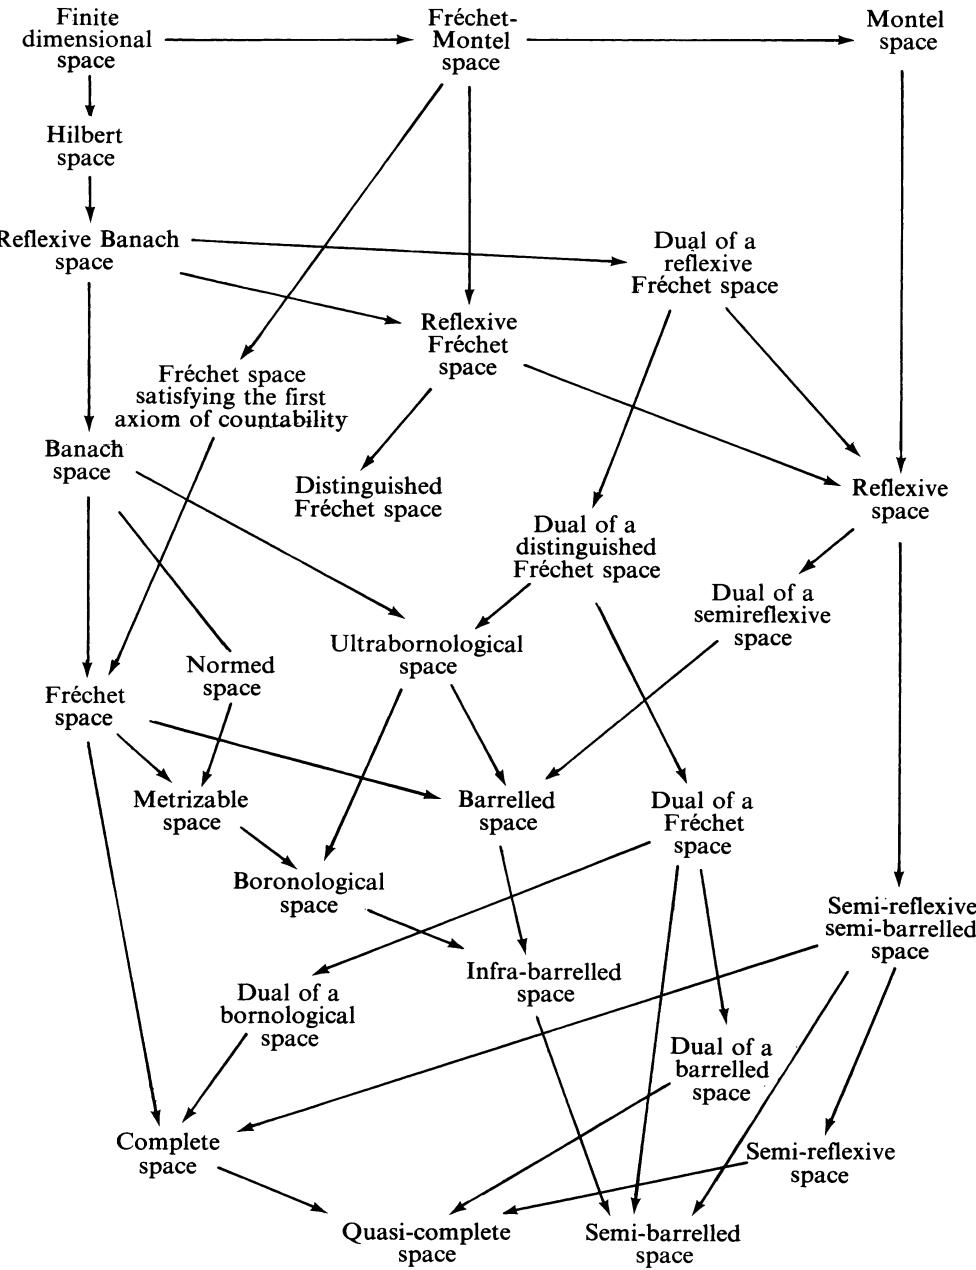
\includegraphics[keepaspectratio]{images/part002_27b26067.jpg}}

\bourbakitable{局部凸空间的对偶上的主要有界结构}{}
\pandocbounded{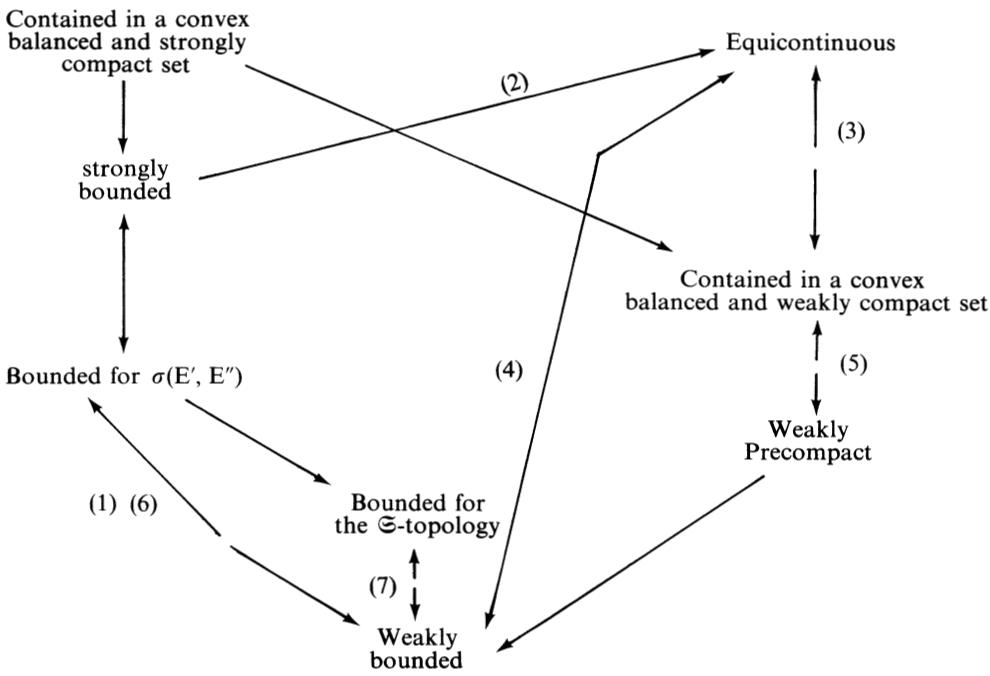
\includegraphics[keepaspectratio]{images/part002_d08e803b.jpg}}

注意 --- 我们用 S 表示 E 的有界子集的这样一个族：其每个元素都含于该族中的某个集合内。箭头旁的数字表示：当同号性质成立时，相应的蕴含关系成立。

\paragraph{性质}

\begin{enumerate}
\def\labelenumi{\arabic{enumi})}
\item
  每当 E 半自反时；
\item
  每当 E 是有界型空间时（III, p.~22, 命题 10）；
\item
  当且仅当 E 具有 Mackey 拓扑 \(\tau(\mathrm{E},\mathrm{E}^{\prime})\) ；
\item
  当且仅当 E 是桶型空间；
\item
  当且仅当 \(\mathbf{E}'\) 对 \(\sigma (\mathbf{E}',\mathbf{E})\) 拟完备
\item
  每当 E 半完备时（更不用说拟完备或完备了）（III, p.~27, 推论 1）；
\item
  每当 \(\mathfrak{S}\) 由闭凸均衡包为半完备的集合组成时（III, p.~27, 定理 2）。
\end{enumerate}

当 E 是 Montel 空间时，上述所有有界结构都相同。

\chapter{\texorpdfstring{希尔伯特空间 \(^{1}\) （初等理论）}{希尔伯特空间 \^{}\{1\} （初等理论）}}

在本章中，K 表示域 R 或域 C。对每个复数 \(\xi = \alpha + i\beta (\alpha, \beta \text{ real}), \overline{\xi}\) 表示共轭 \(\alpha - i\beta\) （\(\xi\) 的）；特别地，\(\overline{\xi} = \xi\) 当且仅当 \(\xi\) 是实数。

\section{准希尔伯特空间与希尔伯特空间}

\subsection{埃尔米特型}

我们回顾《代数》中给出的下述定义（A, IX, § 3, No.~1）：

定义 1. --- 设 E 为域 K 上的向量空间。E 上的（左）埃尔米特型是从 E × E 到 K 中的一个映射 f，它满足下述条件（对 E 中的 \(x_{1}\) 、 \(x_{2}\) 、x、\(y_{1}\) 、 \(y_{2}\) 、y 与 K 中的 \(\lambda\) 、 \(\mu\) ）：

\begin{enumerate}
\def\labelenumi{(\arabic{enumi})}
\tightlist
\item
\item
\end{enumerate}

\[
\begin{array}{c} \left\{ \begin{array}{l} f (x _ {1} + x _ {2}, y) = f (x _ {1}, y) + f (x _ {2}, y) \\ f (x, y _ {1} + y _ {2}) = f (x, y _ {1}) + f (x, y _ {2}) \end{array} \right. \\ \left\{ \begin{array}{l} f (\lambda x, y) = \overline {{\lambda}} f (x, y) \\ f (x, \mu y) = \mu f (x, y) \\ f (x, y) = \overline {{f (y , x)}}  . \end{array} \right. \end{array}\tag{3}
\]

当域 K 是 R 时，E 上的埃尔米特型的概念就化为 \(E \times E\) 上的对称双线性型的概念（A, III, § 6, No.~3）。

我们注意到，条件 (1) 中的第二个与条件 (2) 中的第二个可由其余三个推出。

由 (1) 与 (2) 我们立即得到

\[
f \left(\sum_ {j} \lambda_ {j} x _ {j}, \sum_ {k} \mu_ {k} y _ {k}\right) = \sum_ {j, k} \bar {\lambda} _ {j} \mu_ {k} f \left(x _ {j}, y _ {k}\right).\tag{4}
\]

特别地，若 \(\mathbf{E}\) 是有限维的，且 \((e_j)_{1 \leqslant j \leqslant n}\) 是 \(\mathbf{E}\) 的一个基，则对 \(x = \sum_{j=1}^{n} \xi_j e_j\) 与 \(y = \sum_{j=1}^{n} \eta_j e_j\) ，有

\[
f (x, y) = \sum_ {j, k} \alpha_ {j k} \overline {{{{\xi}}}} _ {j} \eta_ {k}
\]

其中记 \(\alpha_{jk} = f(e_j, e_k)\) ；此外，关系式 (3) 等价于 \(\alpha_{jk} = \overline{\alpha_{kj}}\) 对每对指标 \(j, k\) 成立；这特别蕴含诸数 \(\alpha_{jj}\) 是实数。

由 (3)，数 \(Q(x) = f(x, x)\) 对所有 \(x \in E\) 是实数。此外，我们立即可以建立下列公式，称为极化公式

\begin{enumerate}
\def\labelenumi{(\arabic{enumi})}
\setcounter{enumi}{4}
\tightlist
\item
\end{enumerate}

\[
4 f (x, y) = \sum_ {\varepsilon^ {2} = 1} \varepsilon \mathrm{Q} (x + \varepsilon y) \quad \text { if } \quad \mathbf {K} = \mathbf {R},\tag{6}
\]

\[
4 f (x, y) = \sum_ {\varepsilon^ {4} = 1, \varepsilon \in \mathbf {C}} \varepsilon \mathrm{Q} (x + \overline {{{\varepsilon}}} y) \quad \text { if } \quad \mathbf {K} = \mathbf {C}.
\]

注. --- 我们指出，公式 (6) 对 \(E \times E\) 上的每个半双线性型都成立（也就是说，对每个满足 (1) 与 (2) 但不必满足 (3) 的函数 f 成立）。这个注表明，当 K = C 时，使 \(f(x, x)\) 对所有 \(x \in E\) 为实数的半双线性型 f 必是埃尔米特的：这时关系式 (6) 给出 \(\overline{f(y, x)} = f(x, y)\) ，因为我们有 \(y + \varepsilon x = \varepsilon(x + \overline{\varepsilon}y)\) ，且 \(\mathbf{Q}(\varepsilon z) = \mathbf{Q}(z)\) 对 \(\varepsilon^{4} = 1\) 成立。

由极化公式，我们特别有

命题 1. --- 若 \(f\) 是 \(\mathbf{E}\) 上的埃尔米特型，且 \(\mathbf{M}\) 是 \(\mathbf{E}\) 的一个使 \(f(x, x) = 0\) 对所有 \(x \in \mathbf{M}\) 成立的向量子空间，则也有 \(f(x, y) = 0\) 对每对点 \(x, y\) （\(\mathbf{M}\) 中的）成立。

设 \(f\) 为 \(\mathbf{E}\) 上的埃尔米特型；集 \(\mathbf{N}\) —— 即全体 \(x \in \mathbf{E}\) ，使 \(f(x, y) = 0\) 对所有 \(y \in \mathbf{E}\) 成立 —— 是 \(\mathbf{E}\) 的一个向量子空间。由 (3) 可知，若 \(x_1 \equiv x_2 \pmod{\mathbf{N}}\) 且 \(y_1 \equiv y_2 \pmod{\mathbf{N}}\) ，则有 \(f(x_1, y_1) = f(x_2, y_2)\) ；因此，在商空间 \(\mathrm{E/N}\) 上，我们定义一个半双线性型 \(f\) ，即令 \(\dot{f}(\dot{x}, \dot{y}) = f(x, y)\) （对所有 \(x \in \dot{x}\) 与所有 \(y \in \dot{y}\) ）；显然 \(\dot{f}\) 是埃尔米特的，且关系 \(\langle \dot{f}(\dot{x}, \dot{y}) = 0 \text{ 对所有 } \dot{y} \in \mathrm{E/N} \rangle\) 蕴含 \(\dot{x} = 0 \text{ 于 } \mathrm{E/N}\) ，换言之（A, IX），\(\dot{f}\) 是非退化的。我们说 \(f\) 是与 \(f\) 相伴的非退化埃尔米特型。

\subsection{正埃尔米特型}

定义 2. --- 设 E 为域 K 上的向量空间。E 上的埃尔米特型 f 称为正的，如果 \(f(x, x) \geqslant 0\) 对所有 \(x \in E\) 成立。

显然，向量空间 E 上的全体埃尔米特型构成域 R 上的一个向量空间（当 K 是 C 时，不构成域 C 上的向量空间）：在这个空间中，由定义 2 与命题 1，诸正埃尔米特型构成一个真尖凸锥（II, p.~10）。

命题 2. --- 若 \(f\) 是正埃尔米特型，则有

\[
\left| f (x, y) \right| ^ {2} \leqslant f (x, x) f (y, y)\tag{7}
\]

对 E 中每个 x 与 y（Cauchy-Schwarz 不等式）。

先设 \(f(y, y) \neq 0\) 。对每个 \(\xi \in \mathbf{K}\) ，有

\[
f (y, y) f (x + \xi y, x + \xi y) \geqslant 0
\]

它可写成

\[
f (x, x) f (y, y) - | f (x, y) | ^ {2} + (\xi f (y, y) + \overline {{f (x , y)}}) (\bar {\xi} f (y, y) + f (x, y)) \geqslant 0.
\]

在这个不等式中把 \(\xi\) 换成 \(-\overline{f(x,y)} / f(y,y)\) ，即得 (7)。若 \(f(x,x)\neq 0\) ，论证类似。

最后，若 \(f(x, x) = f(y, y) = 0\) ，则 \(f(x + \xi y, x + \xi y) \geqslant 0\) 对所有 \(\xi \in \mathbf{K}\) 成立，这可写成

\[
\xi f (x, y) + \overline {{{{\xi f (x , y)}}}} \geqslant 0.
\]

在这个不等式中把 \(\xi\) 换成 \(-\overline{f(x,y)}\) ，得 \(-2|f(x,y)|^2 \geqslant 0\) ，从而 \(f(x,y) = 0\) ；在此情形我们同样得到 (7)。

推论 1. --- 若 \(f\) 是正埃尔米特型，则集 \(\mathbf{N}\) —— 即全体 \(x \in \mathbf{E}\) ，使 \(f(x, x) = 0\) —— 与全体 \(x \in \mathbf{E}\) （使 \(f(x, y) = 0\) 对所有 \(y \in \mathbf{E}\) 成立的）组成的向量子空间重合。

推论 2. --- 为使一个正埃尔米特型非退化，必要且充分的是关系 \(x \neq 0\) 蕴含 \(f(x, x) > 0\) 。

这由推论 1 立即得出。

对 E 上的每个正埃尔米特型 f，与 \(f(\mathrm{V}, \mathrm{p.~2})\) 相伴的非退化埃尔米特型显然是 E/N 上的正埃尔米特型。

命题 3. --- 设 f 为 E 上的正埃尔米特型。令

\[
p (x) = f (x, x) ^ {1 / 2}
\]

对所有 \(x \in \mathbb{E}\) 。则 \(p\) 是 \(\mathbb{E}\) 上的半范数，且是范数当且仅当 \(f\) 非退化。只需证明不等式 \(p(x + y) \leqslant p(x) + p(y)\) 。但我们有

\[
f (x + y, x + y) = f (x, x) + f (y, y) + f (x, y) + \overline {{f (x , y)}}
\]

且由 Cauchy-Schwarz 不等式

\[
\begin{array}{c} f (x + y, x + y) \leqslant f (x, x) + f (y, y) + 2 (f (x, x) f (y, y)) ^ {1 / 2} \\ = \bigl (f (x, x) ^ {1 / 2} + f (y, y) ^ {1 / 2} \bigr) ^ {2}. \end{array}\tag{8}
\]

注. --- 1) 假设 \(f\) 是正的且非退化的，并设 \(x, y\) 是两个 \(\neq 0\) 的向量。Cauchy-Schwarz 不等式的证明表明，若 (7) 的两端相等，则存在标量 \(\xi\) 使 \(f(x + \xi y, x + \xi y) = 0\) ，从而 \(x + \xi y = 0\) ，换言之，x 与 y 线性相关；反之是直接的。不等式 (8) 的证明表明，等式 \(p(x + y) = p(x) + p(y)\) 只当 x 与 y 线性相关时才可能成立；若 \(y = \lambda x\) ，前述等式可写成 \(|1 + \lambda| = 1 + |\lambda|\) ，它蕴含 \(\lambda\) 是实数且是正的。

\begin{enumerate}
\def\labelenumi{\arabic{enumi})}
\setcounter{enumi}{1}
\tightlist
\item
  设 \(f\) 为 \(\mathbf{E}\) 上的正埃尔米特型，并给 \(\mathbf{E}\) 赋以半范数 \(x \mapsto f(x, x)^{1/2}\) ；若 \(\dot{f}\) 是定义在 \(\mathrm{E/N}\) 上的与 \(f\) 相伴的正的非退化埃尔米特型，则把范数 \(x \mapsto \hat{f}(\dot{x}, \dot{x})^{1/2}\) 赋予 \(\mathrm{E/N}\) 所得的赋范空间就是与 \(\mathbf{E}\) 相伴的赋范空间（II, p.~5）。
\end{enumerate}

定义 3. --- 设 E 为域 K 上的向量空间。E 上的半范数 p 称为准希尔伯特的，如果存在 E 上的正埃尔米特型 f，使 \(p(x) = f(x, x)^{1/2}\) 对所有 \(x \in E\) 成立。

注意，对 E 上的半范数 p，至多存在一个正埃尔米特型 f，使 \(p(x) = f(x, x)^{1/2}\) 对所有 \(x \in E\) 成立；这由极化公式得出（V, p.~2）。

\subsection{准希尔伯特空间}

定义 4. --- 准希尔伯特空间是一个赋有域 K 上的向量空间结构和一个正埃尔米特型的集合 E。当 K 是 R（相应地，K 是 C）时，我们说 E 是实（相应地，复）准希尔伯特空间。

例. --- 1) 型 \((\lambda, \mu) \mapsto \overline{\lambda}\mu\) 在 K 上定义了一个准希尔伯特结构，称为典范结构。当把 K 看作准希尔伯特空间时，除非另有说明，我们总指它具有这个结构。

\begin{enumerate}
\def\labelenumi{\arabic{enumi})}
\setcounter{enumi}{1}
\tightlist
\item
  设 I 为 R 中的一个区间（有界或无界），E 为定义在 I 上、取值于 C 且具有紧支撑的受控函数（FVR, II, p.~4）组成的集。显然
\end{enumerate}

\(\mathbf{E}\) 是 \(\mathbf{C}\) 上的向量空间；设 \(f\) 为半双线性型 \((x, y) \mapsto \int_{1}^{\infty} \overline{x(t)} y(t) dt\) ；

立即可以看出 \(f\) 是 \(E\) 上的正埃尔米特型，从而在此空间上定义了一个准希尔伯特结构。

\begin{enumerate}
\def\labelenumi{\arabic{enumi})}
\setcounter{enumi}{2}
\tightlist
\item
  设 \(n \geqslant 0\) 为整数。我们在空间 \(\mathbf{K}^n\) 上借助埃尔米特型
\end{enumerate}

\[
(x, y) \mapsto \sum_ {j = 1} ^ {n} \overline {{{{x}}}} _ {j} y _ {j}
\]

定义一个准希尔伯特空间结构（对 \(x = (x_{1}, \ldots, x_{n})\) 与 \(y = (y_{1}, \ldots, y_{n})\) ）。当 \(\mathbf{K}\) 是 \(\mathbf{R}\) 时，我们看到这正是 \(\mathbf{R}^{n}\) 中两个向量的内积（GT, VI, § 2, No.~2）。

* 4) 设 \(\ell^2\) （或 \(\ell^2(\mathbf{N})\) ）为序列 \(x = (x_n)_{n \in \mathbb{N}}\) （元素在 \(\mathbf{K}\) 中且使 \(\sum_{n=0}^{\infty} |x_n|^2\) 为有限）组成的集。可以证明 \(\ell^2\) 是 \(\mathbf{K}^{\mathbf{N}}\) 的向量子空间，并可在其上定义一个准

希尔伯特空间结构于 \(\ell^2\) ，借助埃尔米特型 \((x, y) \mapsto \sum_{n=0}^{\infty} \overline{x}_n y_n\) （参见~V, p.~18）。

\begin{enumerate}
\def\labelenumi{\arabic{enumi})}
\setcounter{enumi}{4}
\tightlist
\item
  设 \(\mathbf{E}\) 为实准希尔伯特空间，\(f\) 为 \(\mathbf{E}\) 上相应的对称双线性型。设 \(\mathrm{E}_{(\mathbf{C})}\) 为 \(\mathbf{E}\) 的向量空间复化；把 \(\mathbf{E}\) 等同于 \(\mathrm{E}_{(\mathbf{C})}\) 的一个子集（借助映射 \(x \mapsto 1 \otimes x\) ），使 \(\mathrm{E}_{(\mathbf{C})}\) 的每个元素都可唯一地写成 \(x_1 + ix_2\) ，其中 \(x_1, x_2\) 属于 \(\mathbf{E}\) 。映射 \(f\) 唯一地延拓为一个埃尔米特型 \(f_{(\mathbf{C})}\) （\(\mathrm{E}_{(\mathbf{C})}\) 上的）；我们有，
\end{enumerate}

\[
f _ {(\mathbf {C})} \left(x _ {1} + i x _ {2}, y _ {1} + i y _ {2}\right) = f \left(x _ {1}, y _ {1}\right) + f \left(x _ {2}, y _ {2}\right) + i \left(f \left(x _ {1}, y _ {2}\right) - f \left(x _ {2}, y _ {1}\right)\right).
\]

特别地，我们有

\[
f _ {(\mathbf {C})} (x _ {1} + i x _ {2}, x _ {1} + i x _ {2}) = f (x _ {1}, x _ {1}) + f (x _ {2}, x _ {2}) \geqslant 0,
\]

因此 \(f_{(\mathbf{C})}\) 是正的。我们说 \(\mathrm{E}_{(\mathbf{C})}\) （赋有 \(f_{(\mathbf{C})}\) ）是 \(\mathbf{E}\) 的准希尔伯特空间复化。

每当只考虑向量空间 E 上的一个准希尔伯特空间结构时，对 E 的一对点 \((x, y)\) ，定义该结构的埃尔米特型在这对点上的值记作 \(\langle x|y\rangle_{E}\) ，或在不致混淆时简记为 \(\langle x|y\rangle\) 。这个数称为 x 与 y 的内积 \(^{1}\) （当 y = x 时称为 x 的标量平方）。向量 x, y 称为正交的，如果 \(\langle x|y\rangle = 0\) 。函数 \(x \mapsto \|x\| = \langle x|x\rangle^{1/2}\) 是向量空间 E 上的半范数（V, p.~3）；准希尔伯特空间总是被认为赋有这个半范数（从而也赋有相应的拓扑与一致结构）。

采用这些记号，在准希尔伯特空间 E 中，Cauchy-Schwarz 不等式可写成

\[
\left| \langle x | y \rangle \right| \leqslant \| x \|\cdot \| y \|.\tag{9}
\]

因此，内积是 \(\mathbf{E} \times \mathbf{E}\) 上的连续半双线性型（II, p.~5, 命题 4）。

为使 E 是 Hausdorff 的，必要且充分的是 \(x \mapsto \|x\|\) 是 E 上的范数；换言之，埃尔米特型 \((x, y) \mapsto \langle x | y \rangle\) 是正的且非退化的；这等价于说 0 是 E 中唯一与自身正交的向量。

按照一般定义（S, IV, § 1, No.~5），准希尔伯特空间 E 到准希尔伯特空间 F 上的同构是从 E 到 F 上的一个双射线性映射 u，它满足

\[
\langle u (x) | u (y) \rangle = \langle x | y \rangle\tag{10}
\]

对 E 中每个 x 与 y。由此推出，\(\|u(x)\| = \|x\|\) 对所有 \(x \in E\) 成立，且 u 显然是 E 与 F 的拓扑向量空间结构之间的同构；若 E 与 F 是 Hausdorff 的，则 u 是 E 到 F 上的一个等距。反之，若 u 是从 E 到 F 上的双射线性映射，且 \(\|u(x)\| = \|x\|\) 对所有 \(x \in E\) 成立，则极化公式（V, p.~2）表明 u 是 E 到 F 上的准希尔伯特空间同构。

设 \(E\) 为复准希尔伯特空间，\(\langle x|y\rangle\) 为 \(E\) 中的内积。在集合 \(E\) 上，可以定义关于 \(C\) 的第二个向量空间结构，取同样的加法群规律，并以 \((\lambda, x) \mapsto \overline{\lambda}x\) 为外合成规律（A, II, § 1, No.~13）；对这个向量空间结构，\((x, y) \mapsto \langle y|x\rangle\) 是一个正埃尔米特

\(^{1}\) 有时我们会用 \((x|y)\) 表示 \(\langle y|x\rangle\) 。注意 V, p.~2 的公式 (4) 取下列等价形式：

(4')

\[
\langle \sum_ {i} \lambda_ {i} x _ {i} | \sum_ {j} \mu_ {j} y _ {j} \rangle = \sum_ {i, j} \overline {{{{\lambda}}}} _ {i} \mu_ {j} \langle x _ {i} | y _ {j} \rangle .\tag{4"}
\]

\[
(\sum_ {i} \lambda_ {i} x _ {i} | \sum_ {j} \mu_ {j} y _ {j}) = \sum_ {i, j} \lambda_ {i} \overline {{\mu}} _ {j} (x _ {i} | y _ {j}).
\]

型。给 E 赋以这个新的向量空间结构与新的埃尔米特型所得的准希尔伯特空间 \(\overline{E}\) 称为 E 的共轭空间。E 到 \(\overline{E}\) 上的同构 u 是 E 到自身的一个半线性映射（关于 C 的自同构 \(\xi \mapsto \overline{\xi}\) ），满足 \(\langle u(y)|u(x)\rangle = \langle x|y\rangle\) 或 \(\langle u(x)|u(y)\rangle = \overline{\langle x|y\rangle}\) （对 E 中的 x, y）；这样的映射称为准希尔伯特空间 E 的半自同构。

若 E 是准希尔伯特空间，M 是 E 的向量子空间，则内积 \(\langle x|y\rangle\) 在 \(M \times M\) 上的限制是 M 上的正埃尔米特型，从而在 M 上定义了一个准希尔伯特空间结构；我们说这个结构由 E 的结构诱导，或说 M 是 E 的准希尔伯特子空间。

\subsection{希尔伯特空间}

定义 5. --- 希尔伯特空间（或 Hilbert 空间）是 Hausdorff 且完备的准希尔伯特空间。我们说向量空间 E（K 上的）上的范数是希尔伯特的，如果它是准希尔伯特的，且赋范空间 E 是完备的。

若 E 是希尔伯特空间且 M 是 E 的闭向量子空间，则 M 上诱导的准希尔伯特空间结构实际上是希尔伯特空间结构。这时我们说赋有诱导结构的 M 是 E 的希尔伯特子空间。

例. --- 1) V, p.~4 的例 1、3、4 中定义的准希尔伯特空间都是希尔伯特空间。另一方面，例 2 中定义的准希尔伯特空间既非 Hausdorff，也非完备。希尔伯特空间的复化是希尔伯特空间。

* 2) 设 X 为 Hausdorff 拓扑空间，\(\mu\) 为 X 上的正测度。设 \(L^2(X, \mu)\) 为 X 上取值于 C 的全体平方 \(\mu\) -可积函数按 \(\mu\) 的等价类组成的空间。这是一个复希尔伯特空间，其内积由下式给出

\[
\langle f | g \rangle = \int_ {\mathrm{X}} \overline {{{f (x)}}} g (x) d \mu (x). *
\]

* 3) 设 \(n \geqslant 1\) 为整数，\(U\) 为 \(\mathbf{R}^n\) 中的开集。设 \(\mu\) 为 \(U\) 上由 \(\mathbf{R}^n\) 上的 Lebesgue 测度诱导的测度，令 \(\mathcal{H}^0 = L^2(U, \mu)\) 。用 \(\mathcal{H}^1\) 表示具有下列性质的所有函数 \(f \in \mathcal{H}^0\) 组成的空间；对 \(1 \leqslant i \leqslant n\) ，存在函数 \(g_i \in \mathcal{H}^0\) 使

\[
\int_ {\mathrm{U}} g _ {i} (x) h (x) d \mu (x) = - \int_ {\mathrm{U}} f (x) \mathrm{D} _ {i} h (x) d \mu (x)
\]

对每个函数 \(h\) （\(\mathbf{C}^1\) 类的，在 \(\mathbf{U}\) 中有紧支撑的）成立。函数 \(g_i\) 在相差一个关于 \(\mu\) 的等价类的意义下唯一确定，记作 \(\mathbf{D}_i f\) 或 \(\partial f / \partial x_i\) （第 i 个偏导数）。对整数 \(s \geqslant 1\) 用归纳法，把 \(\mathcal{H}^s\) 定义为所有函数 \(f \in \mathcal{H}^1\) （使 \(D_i f \in \mathcal{H}^{s-1}\) 对 \(1 \leqslant i \leqslant n\) 成立的）组成的集。我们用下列公式在 \(\mathcal{H}^s\) 上定义内积

\[
\langle f | g \rangle = \sum_ {k = 0} ^ {s} \sum_ {1 \leqslant i _ {1} \leqslant \dots \leqslant i _ {k} \leqslant n} \int \overline {{{{\mathrm{D} _ {i _ {1}} \dots \mathrm{D} _ {i _ {k}} f}}}}. \mathrm{D} _ {i _ {1}} \dots \mathrm{D} _ {i _ {k}} g d \mu .
\]

于是 \(\mathcal{H}^s\) 是一个复希尔伯特空间，称为指标 \(s\) 的 Sobolev 空间。

* 4) 设 X 为 \(\mathbf{C}^r\) 类（\(r \geqslant 1\) ）纯的、维数有限为 \(n\) 的微分流形。

在向量纤维空间 \(\Lambda^{n}\mathrm{T}(\mathrm{X})\) 中，设 L 为零截面的余集。对每个实数 \(\lambda \neq 0\) ，映射 \(u \mapsto \lambda u\) （从 \(\Lambda^{n}\mathrm{T}(\mathrm{X})\) 到自身的）使 L 稳定。

设 \(\alpha\) 为复数。一个复值函数 \(\omega\) （定义在 \(\mathbf{L}\) 上），若 \(\omega (\lambda u) = |\lambda |^{\alpha}\omega (u)\) 对 \(u\in \mathbf{L}\) 与任意非零实数 \(\lambda\) 成立，就称为 \(\alpha\) 阶密度（\(\mathbf{X}\) 上的）。我们说 1 阶密度 \(\omega\) 是局部可积的，如果存在一个开覆盖 \((\mathrm{U}_i)_{i\in \mathbf{I}}\) （\(\mathbf{X}\) 的），且对每个 \(i\in \mathbf{I}\) ，存在一个坐标系 \(\xi_i = (\xi_i^1,\dots,\xi_i^n)\) （\(\mathrm{U}_i\) 上的）与一个复值函数 \(f_{i}\) （\(\xi_i(\mathrm{U}_i)\) 上的），满足下列条件：a) 函数 \(f_{i}\) 在开集 \(\xi_i(\mathrm{U}_i)\) （\(\mathbf{R}^n\) 中的）上关于 Lebesgue 测度 \(\mu\) 是局部可积的；

\begin{enumerate}
\def\labelenumi{\alph{enumi})}
\setcounter{enumi}{1}
\tightlist
\item
  设 \(x \in \mathbf{U}_i\) ；若 \((\partial_{1,i,x}, \ldots, \partial_{n,i,x})\) 是 \(\mathrm{T}_x\mathrm{X}\) 的、与坐标系 \((\xi_i^1, \ldots, \xi_i^n)\) （\(\mathbf{U}_i\) 中的）相伴的基，则有
\end{enumerate}

\[
\omega \left(\partial_ {1, i, x} \wedge \dots \wedge \partial_ {n, i, x}\right) = f _ {i} \left(\xi_ {i} ^ {1} (x), \dots , \xi_ {i} ^ {n} (x)\right).
\]

于是，存在唯一的测度 \(\tilde{\omega}\) （\(\mathbf{X}\) 上的），使对每个 \(i\in \mathrm{I}\) ，在 \(\xi_{i}\) 下 \(\tilde{\omega}\) 在 \(\mathrm{U}_i\) 上的限制的像等于测度 \(f_{i}.\mu\) （参见~VAR, R, 10.4.3）。

设 \(\mathcal{V}\) （相应地，\(\mathcal{N}\) ）为由可测密度 \(\omega\) （\(1/2\) 阶）组成的、使与 1 阶密度 \(|\omega|^2\) 相伴的测度有界（相应地，为零）的向量空间。设 \(\omega_1\) 与 \(\omega_2\) 属于 \(\mathcal{V}\) ；则 \(\omega = \overline{\omega}_1\omega_2\) 是 1 阶密度，且测度 \(\tilde{\omega}\) （与 \(\omega\) 相伴的）有界；数 \(\int_{\mathbf{X}}\tilde{\omega}\) 只依赖于类 \(\dot{\omega}_1\) 与 \(\dot{\omega}_2\) （即 \(\omega_1\) 与 \(\omega_2\) 模 \(\mathcal{N}\) 的类），记作 \(\langle\omega_1|\omega_2\rangle\) 或 \(\langle\dot{\omega}_1|\dot{\omega}_2\rangle\) 。于是映射 \((\dot{\omega}_1,\dot{\omega}_2)\mapsto\langle\dot{\omega}_1|\dot{\omega}_2\rangle\) 给向量空间 \(\Omega_{1/2}(\mathbf{X})=\mathcal{V}/\mathcal{N}_{*}\) 赋以一个复希尔伯特空间结构。

*5) 设 D 为 C 中以 0 为心、1 为半径的开圆盘。Hardy 空间 \(\mathrm{H}^2 (\mathbf{D})\) 由满足下列条件的全纯函数 \(f\colon \mathbf{D}\to \mathbf{C}\) 组成：

\[
\sup _ {0 <   \mathbf {R} <   1} \int_ {0} ^ {1} | f (\mathbf {R}. \mathbf {e} (\theta)) | ^ {2} d \theta <   + \infty .
\]

若 \(f_{1}\) 与 \(f_{2}\) 属于 \(\mathrm{H}^2 (\mathbf{D})\) ，则极限

\[
\langle f _ {1} | f _ {2} \rangle = \lim _ {\mathbf {R} \rightarrow 1} \int_ {0} ^ {1} \overline {{{f _ {1} (\mathbf {R} . \mathbf {e} (\theta))}}}. f _ {2} (\mathbf {R}. \mathbf {e} (\theta)) d \theta
\]

存在；映射 \((f_1, f_2) \mapsto \langle f_1 | f_2 \rangle\) 给向量空间 \(\mathbf{H}^2(\mathbf{D})\) 赋以一个复希尔伯特空间结构。

为使函数 \(f: \mathbf{D} \to \mathbf{C}\) 属于 \(\mathbf{H}^2(\mathbf{D})\) ，必要且充分的是存在复数的序列 \((a_n)_{n \in \mathbb{N}}\) ，使 \(\sum_{n=0}^{\infty} |a_n|^2 < +\infty\) 且

\[
f (z) = \sum_ {n = 0} ^ {\infty} a _ {n} z ^ {n}
\]

对所有 \(z \in \mathbf{D}\) 成立。这时有 \(\| f\|^2 = \sum_{n=0}^{\infty} |a_n|^2\) ，由此给出从 \(\mathrm{H}^2(\mathrm{D})\) 到希尔伯特空间 \(\ell^2\) 上的一个同构（V, p.~4）。 *

每个 Hausdorff 准希尔伯特空间都同构于一个在相差一个同构的意义下确定的希尔伯特空间的处处稠密子空间。确切地说：

命题 4. --- 设 E 为 Hausdorff 准希尔伯特空间，\(\hat{E}\) 为 E 的赋范空间完备化（GT, IX, § 3, No.~3）。内积 \((x, y) \mapsto \langle x|y \rangle\) 由连续性延拓为 \(\hat{\mathbf{E}}\) 上的正且非退化的埃尔米特型，并在 \(\hat{\mathbf{E}}\) 上定义一个希尔伯特空间结构。

\((x, y) \mapsto \langle x|y \rangle\) 到 \(\hat{E} \times \hat{E}\) 上的延拓的存在性由这个半双线性型在 \(E \times E\) 上的连续性得出（GT, III, §6, No.~5, 定理 1）。此外，这个延拓（仍记作 \((x, y) \mapsto \langle x|y \rangle\) ）是埃尔米特型且满足关系 \(\langle x|x\rangle = \|x\|^2\) ，这由恒等式延拓原理得出（ \(\|x\|\) 是 \(\hat{E}\) 上把 E 上的范数用连续性延拓所得的范数）；这就证明了关系 \(\langle x|x\rangle = 0\) 蕴含在 \(\hat{E}\) 中 x = 0，从而型 \((x, y) \mapsto \langle x|y \rangle\) 是正的且非退化的，于是在 \(\hat{E}\) 上定义一个希尔伯特空间结构。

证毕。

这个希尔伯特空间称为 Hausdorff 准希尔伯特空间 E 的完备化。

* 例 6. --- 设 U 为 \(\mathbf{R}^n\) 的开子集（ \(n \geqslant 1\) ）。设 \(\mathcal{C}_0^1(\mathrm{U})\) 为 U 中具有紧支撑的 \(\mathbf{C}^1\) 类函数全体组成的向量空间。我们在 \(\mathcal{C}_0^1(\mathrm{U})\) 上定义一个 Hausdorff 准希尔伯特空间结构，其内积由下式给出

\[
\langle f | g \rangle = \sum_ {i = 1} ^ {n} \int_ {\mathrm{U}} \overline {{{{\mathbf {D} _ {i} f (x)}}}}. \mathbf {D} _ {i} g (x) d x.
\]

这个准希尔伯特空间不完备。它的完备化称为与 U 相伴的 Dirichlet 空间。 *

推论. --- 设 V 为 K 上的向量空间，f 为 V 上的正埃尔米特型。a) 存在一个 Hilbert 空间 E 和一个线性映射 \(u:V \rightarrow E\) ，使 \(f(x,y) = \langle u(x)|u(y) \rangle\) 对 V 中的 x, y 成立，且使 \(u(V)\) 在 E 中稠密。

\begin{enumerate}
\def\labelenumi{\alph{enumi})}
\setcounter{enumi}{1}
\tightlist
\item
  若两个偶 \((\mathbf{E}_{i}, u_{i})\) 满足与 a) 类似的条件，则存在唯一的同构 \(\phi\) （从 Hilbert 空间 \(E_{1}\) 到 Hilbert 空间 \(E_{2}\) 上的）使 \(u_{2} = \phi \circ u_{1}\) 。
\end{enumerate}

设 N 为全体 \(x \in V\) （使 \(f(x, x) = 0\) 的）组成的集。我们在空间 V/N 上用 \(\langle \dot{x} | \dot{y} \rangle = f(x, y)\) （对 \(x \in \dot{x}\) 与 \(y \in \dot{y}\) ）定义一个正且非退化的埃尔米特型。设 E 为 V/N 的希尔伯特空间完备化，u 为从 V 到 E 中的映射 \(x \mapsto x + N\) 。于是 a) 的条件满足。

在 b) 的假设下，N 等于 \(u_{1}\) 的核，也等于 \(u_{2}\) 的核。因此存在双射线性映射 \(\phi_{0}\) （从 \(u_{1}(V)\) 到 \(u_{2}(V)\) 上的），使 \(u_{2}(x) = \phi_{0}(u_{1}(x))\) 对所有 \(x \in V\) 成立。立即可以验证 \(\phi_{0}\) 是准希尔伯特空间之间的同构，从而是一个等距。由于对 i = 1, 2，\(u_{i}(V)\) 在 \(E_{i}\) 中稠密，\(\phi_{0}\) 唯一地延拓为一个等距 \(\phi\) （从 \(E_{1}\) 到 \(E_{2}\) 上的），由此得 b)。

我们说希尔伯特空间 \(\mathbf{E}\) 是 \(\mathbf{V}\) 的分离完备化（关于型 \(f\) ）。

例 7. --- 设 G 为一个群（单位元为 1），\(\pi\) 为从 G 到一个复希尔伯特空间 E 的自同构群中的同态；我们说 \(\pi\) 是 G 在 E 中的一个酉表示。设 \(a \in E\) ；我们令

\[
\phi (x) = \langle a | \pi (x). a \rangle
\]

对所有 \(x \in \mathbf{G}\) 成立。则 \(\phi : \mathbf{G} \to \mathbf{C}\) 是正定的，换言之满足关系：

(PD) 对 C 中每个 \(\lambda_{1},\ldots,\lambda_{n}\) 与 G 中每个 \(x_{1},\ldots,x_{n}\) ，有

\[
\sum_ {i, j = 1} ^ {n} \overline {{\lambda}} _ {i} \lambda_ {j} \phi (x _ {i} ^ {- 1} x _ {j}) \geqslant 0.\tag{11}
\]

事实上，(11) 的左端正是 \(\| \sum_{i=1}^{n} \lambda_i \pi(x_i). a \|^2\) 。

反之，设 \(\phi\) 为 \(G\) 上的正定函数。设 \(\mathbf{C}^{(G)}\) 为 \(G\) 上具有有限支撑的全体函数组成的向量空间。我们定义一个埃尔米特型 \(\Phi\) 于 \(G\) 上：

\[
\Phi (u, v) = \sum_ {x, y \in G} \overline {{u (x)}} v (y) \phi (x ^ {- 1} y)\tag{12}
\]

而关系式 (PD) 表明 \(\Phi\) 是正的。由命题 4 的推论，存在一个希尔伯特空间 \(E\) 和一个线性映射 \(\rho : \mathbf{C}^{(G)} \to E\) ，其像稠密，使得

\[
\Phi (u, v) = \langle \rho (u) | \rho (v) \rangle \quad \text { for } \quad u, v \quad \text { in } \quad \mathbf {C} ^ {(G)}.\tag{13}
\]

对每个 \(x \in \mathbf{G}\) ，设 \(\gamma_x\) 为 \(x\) 在 \(\mathbf{C}^{(\mathrm{G})}\) 中的左平移，由 \(\gamma_x u(y) = u(x^{-1}y)\) （对 \(u \in \mathbf{C}^{(\mathrm{G})}\) 与 \(y \in \mathbf{G}\) ）定义。我们有 \(\Phi(\gamma_x u, \gamma_x v) = \Phi(u, v)\) 。现在把命题 4 的推论的断言 \(b\) 应用于 \(\rho\) 与 \(\rho \circ \gamma_x\) ：存在唯一的自同构 \(\pi(x)\) （希尔伯特空间 \(E\) 上的）使 \(\rho \circ \gamma_x = \pi(x) \circ \rho\) 。立即可以看出 \(\pi\) 是从 \(G\) 到 \(E\) 的自同构群中的同态。

设 \(\delta\) 为 \(\mathbf{C}^{(\mathrm{G})}\) 中由 \(\delta(1) = 1\) 与 \(\delta(x) = 0\) （对 \(x \neq 1\) ，\(\mathbf{G}\) 中的）定义的元素。我们有 \(u = \sum_{x \in \mathbf{G}} u(x) \cdot \gamma_x \delta\) 对所有 \(u \in \mathbf{C}^{(\mathrm{G})}\) 成立，于是 \(\rho(u) = \sum_{x \in \mathbf{G}} u(x) \pi(x) \cdot a\) （令 \(a = \rho(\delta)\) ）。公式 (12) 与 (13) 蕴含 \(\phi(x) = \langle a | \pi(x) \cdot a \rangle\) 对所有 \(x \in \mathbf{G}\) 成立。我们注意，向量 \(\pi(x) \cdot a\) （对所有 \(x \in \mathbf{G}\) ）组成的集在 \(\mathbf{E}\) 中是完全的。

\subsection{准希尔伯特空间的凸子集}

若对准希尔伯特空间 E 的任意两点 x, y 计算 \(\|x - y\|^{2} = \langle x - y|x - y \rangle\) 与 \(\|x + y\|^{2} = \langle x + y|x + y \rangle\) ，立即得到«中线恒等式»

\[
\left\| \frac {1}{2} (x + y) \right\| ^ {2} + \left\| \frac {1}{2} (x - y) \right\| ^ {2} = \frac {1}{2} (\| x \| ^ {2} + \| y \| ^ {2}).\tag{14}
\]

由这个恒等式我们导出下列命题：

\pandocbounded{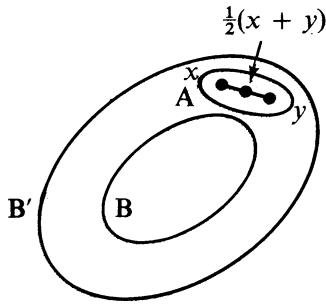
\includegraphics[keepaspectratio]{images/part002_56de9e6b.jpg}}\\
图 1.

命题 5. --- 设 E 为准希尔伯特空间。设 d 为实数 \textgreater0，δ 为使 \(0 \leqslant \delta \leqslant d\) 的实数。设 B 与 B' 为 E 的子集，分别由 \(\|x\| < d\) 与 \(\| x\| \leqslant d + \delta\) 定义，并设 A 为含于 \(\mathbf{B}' - \mathbf{B}\) 的凸集。则对 A 的每对点 \(x, y\) ，有 \(\| x - y\| \leqslant \sqrt{12d\delta}\) （图~1）。

事实上，我们有 \(\frac{1}{2} (x + y)\in \mathbf{A}\) ，故 \(\| \frac{1}{2} (x + y)\| \geqslant d\) ；于是由 (14) 得不等式

\[
\left\| \frac {1}{2} (x - y) \right\| ^ {2} = \frac {1}{2} \left(\| x \| ^ {2} + \| y \| ^ {2}\right) - \left\| \frac {1}{2} (x + y) \right\| ^ {2} \leqslant (d + \delta) ^ {2} - d ^ {2} \leqslant 3 d \delta
\]

由此即得命题。

定理 1. --- 设 E 为准希尔伯特空间，H 为 E 的一个非空凸子集，使得 H 是 E 的 Hausdorff 且完备的一致子空间。对每个 \(x \in E\) ，在 H 中存在唯一的点 \(p_{\mathrm{H}}(x)\) 使 \(\|x - p_{\mathrm{H}}(x)\| = \inf_{y \in \mathrm{H}} \|x - y\|\) 。H 的元素 \(p_{\mathrm{H}}(x)\) 也是 H 中满足关系式 \(^{1}\) 的唯一元素 a

\[
\mathcal {R} \langle x - a | y - a \rangle \leqslant 0\tag{15}
\]

对所有 \(y \in \mathbf{H}\) 成立。

\pandocbounded{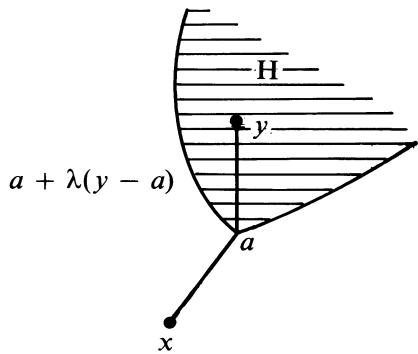
\includegraphics[keepaspectratio]{images/part002_6909685c.jpg}}\\
图 2.

令 \(d = \inf_{y \in \mathbf{H}} \| x - y \|\) ，且对每个整数 \(n > 0\) ，设 \(\mathrm{H}_n\) 为点 \(y\) （在 \(\mathbf{H}\) 中，使 \(\| x - y \| \leqslant d + n^{-1}\) ）所成的集。集 \(\mathrm{H}_n\) 在 \(\mathbf{H}\) 中是闭的，是凸的且非空，且由命题 5，其直径以 \(\sqrt{12d / n}\) 为界（对所有足够大的 \(n\) ）。由于序列 \((\mathrm{H}_n)_{n \geqslant 1}\) 递减，且集 \(\mathbf{H}\) 是 Hausdorff 且完备的，因此 Cauchy 滤子 \((\mathrm{H}_n)_{n \geqslant 1}\) 的基收敛到一点 \(p_{\mathbf{H}}(x)\) （属于 \(\mathbf{H}\) ）；我们有 \(\{p_{\mathbf{H}}(x)\} = \bigcap_{n \geqslant 1} \mathrm{H}_n\) ，故 \(p_{\mathbf{H}}(x)\) 是唯一的点 \(a\) （在 \(\mathbf{H}\) 中），使 \(\| x - a \| = d\) 。

\(^{1}\) 我们回顾（GT, VIII, § 1, No.~1），\(\mathcal{R}(z)\) 表示复数 z 的实部；若 z 是实数，则有 \(\mathcal{R}(z)=z\) 。

设 \(y \in H\) ；由于 \(H\) 是凸的，点 \(z(\lambda) = p_{\mathbf{H}}(x) + \lambda(y - p_{\mathbf{H}}(x))\) （\(E\) 中的）属于 \(H\) ，对每个实数 \(\lambda\) （满足 \(0 < \lambda < 1\) 的）。因此我们有

\[
\left\| x - z (\lambda) \right\| ^ {2} \geqslant \left\| x - p _ {\mathrm{H}} (x) \right\| ^ {2} \quad \text { for } \quad 0 <   \lambda <   1,
\]

由此给出

\[
\mathcal {R} \left\langle x - p _ {\mathrm{H}} (x) \mid y - p _ {\mathrm{H}} (x) \right\rangle = \lim _ {\lambda \rightarrow 0} \frac {1}{2 \lambda} \left\{\| x - p _ {\mathrm{H}} (x) \| ^ {2} - \| x - z (\lambda) \| ^ {2} \right\} \leqslant 0.
\]

反之，设 \(a\) 为 \(\mathbf{H}\) 的一点，使 \(\mathcal{R}\langle x - a|y - a\rangle \leqslant 0\) 对所有 \(y\in \mathbf{H}\) 成立。对每个 \(y\in \mathbf{H}\) ，有

\[
\left\| x - y \right\| ^ {2} = \left\| x - a \right\| ^ {2} + \left\| y - a \right\| ^ {2} - 2 \mathcal {R} \langle x - a | y - a \rangle \geqslant \left\| x - a \right\| ^ {2},
\]

于是 \(\| x - a\| = d\) ，最后由证明的第一部分得出 \(a = p_{\mathrm{H}}(x)\) 。证毕。

在下面，E 到 H 中的映射 \(p_{H}\) 将称为从 E 到 H 上的投影。我们注意 \(p_{\mathrm{H}}(x)=x\) 对所有 \(x\in H\) 成立。

定理 1 的第一部分在关于空间 E 的更一般假设下仍然成立（V, p.~67, 练习 31）。

定理 1 的证明特别建立了下列性质：

推论 1. --- 设 I 为被滤子 \(\mathfrak{F}\) 定向的集合，\((y_i)_{i\in I}\) 为 H 的点的一个族。设 \(x\in E\) 。假设我们有

\[
\lim _ {i, \mathfrak {F}} \| x - y _ {i} \| = \inf _ {z \in \mathrm{H}} \| x - z \|.
\]

则 \(y_{i}\) 趋于 \(p_{\mathrm{H}}(x)\) （关于滤子 \(\mathfrak{F}\) ）。

推论 2. --- 对 E 中每个 x, y，有

\[
\left\| p _ {\mathrm{H}} (x) - p _ {\mathrm{H}} (y) \right\| \leqslant \left\| x - y \right\|.
\]

特别地，从 E 到 H 中的映射 \(p_{H}\) 是连续的。

设 \(x, y\) 为 \(E\) 的两点。令 \(a = p_{\mathrm{H}}(x) - x\) ，\(b = p_{\mathrm{H}}(y) - p_{\mathrm{H}}(x)\) ，\(c = y - p_{\mathrm{H}}(y)\) 。由公式 (15)（V, p.~10）我们有 \(\mathcal{R}\langle a|b\rangle \geqslant 0\) 与 \(\mathcal{R}\langle c|b\rangle \geqslant 0\) 。我们还有 \(a + b + c = y - x\) ，由此给出

\[
\| x - y \| ^ {2} = \| a + b + c \| ^ {2} = \| b \| ^ {2} + \| a + c \| ^ {2} + 2 \mathscr {R} \langle a | b \rangle + 2 \mathscr {R} \langle c | b \rangle
\]

\[
\geqslant \| b \| ^ {2} = \left\| p _ {\mathrm{H}} (x) - p _ {\mathrm{H}} (y) \right\| ^ {2}.
\]

这就证明了推论 2。

命题 6. --- 设 E 为准希尔伯特空间，\(\Phi\) 为由 E 的非空、Hausdorff 且完备的凸子集组成的非空递减有向集。对每个 \(x \in \mathrm{E}\) 与 E 的每个子集 H，令 \(d(x, \mathrm{H}) = \inf_{z \in \mathrm{H}} \| x - z \|\) 。为使属于 \(\Phi\) 的诸集 H 的交 M 非空，必要且充分的是存在 E 中的 \(x_0\) 使 \(\sup_{\mathbf{H} \in \Phi} d(x_0, \mathbf{H})\) 有限。这时对每个 \(x \in \mathbf{E}\) 我们有

\(p_{\mathbf{M}}(x) = \lim_{\mathrm{H}\in \Phi}p_{\mathrm{H}}(x)\) （关于有向集 \(\Phi\) 的极限）。

若 \(\mathbf{M}\) 非空，则 \(d(x,\mathrm{H})\leqslant d(x,\mathbf{M})\) 对所有 \(\mathbf{H}\in \Phi\) 与所有 \(x\in \mathbb{E}\) 成立。

反之，假设存在一点 \(x_0\) （在 \(\mathbf{E}\) 中）与实数 \(\mathbf{C} \geqslant 0\) ，使 \(d(x_0, \mathbf{H}) \leqslant \mathbf{C}\) 对所有 \(\mathbf{H} \in \Phi\) 成立。设 \(x \in \mathbf{E}\) ；则

\[
d (x, \mathrm{H}) \leqslant \| x - x _ {0} \| + \mathrm{C} \quad \text { for   all } \quad \mathrm{H} \in \Phi ,
\]

于是数 \(d = \sup_{\mathbf{H} \in \Phi} d(x, \mathbf{H})\) 有限。设 \(\mathbf{B}\) 为全体 \(z \in E\) （使 \(\| x - z\| \leqslant d\) 的）组成的集。由于 \(\mathbf{B}\) 在 \(\mathbf{E}\) 中是凸的且闭的，故诸集 \(\mathrm{H} \cap \mathrm{B}\) （当 \(\mathrm{H}\) 取遍 \(\Phi\) ）是凸的、Hausdorff 的且完备的。设 \(\varepsilon > 0\) ；存在集 \(\mathrm{H} \in \Phi\) 使 \(d(x, \mathrm{H}) \geqslant \mathrm{d} - \varepsilon\) ，且若 \(\varepsilon < d/2\) ，则 \(\mathrm{H} \cap \mathrm{B}\) 的直径由命题 5（V, p.~9）以 \(\sqrt{12\varepsilon(d - \varepsilon)}\) 为界。换言之，对所有 \(\mathrm{H}_0 \in \Phi\) ，诸闭集 \(\mathrm{H} \cap \mathrm{B}\) （\(\mathrm{H} \in \Phi\) 且 \(\mathrm{H} \subset \mathrm{H}_0\) ）构成 Hausdorff 完备空间 \(\mathrm{H}_0\) 上 Cauchy 滤子的一个基。因此诸集 \(\mathrm{H} \cap \mathrm{B}\) （对 \(\mathrm{H} \in \Phi\) ）的交化为一点 \(y\) 。我们得到 \(y \in \mathbf{M}\) 与 \(\| x - y \| = d = d(x, \mathbf{M})\) 。由于 \(\mathbf{M}\) 在 \(\mathrm{H}_0\) 中是闭的，它是 \(\mathbf{E}\) 中 Hausdorff、凸且完备的集，故 \(y = p_{\mathbf{M}}(x)\) 。对每个 \(\mathrm{H} \in \Phi\) ，我们有 \(p_{\mathrm{H}}(x) \in \mathrm{H} \cap \mathrm{B}\) ，由此得出 \(p_{\mathbf{M}}(x) = \lim_{\mathrm{H} \in \Phi} p_{\mathrm{H}}(x)\) 。

命题 7. --- 设 E 为 Hausdorff 准希尔伯特空间，\(\Psi\) 为由 E 的非空、凸、完备子集组成的非空递增有向集。令 \(A = \bigcup_{H \in \Psi} H\)

并假设闭包 \(\mathbf{N}\) （\(\mathbf{A}\) 的）是完备的。则 \(\mathbf{N}\) 是凸的，且 \(p_{\mathrm{N}}(x) = \lim_{\mathrm{H}\in \Psi}p_{\mathrm{H}}(x)\) 对所有 \(x\in \mathrm{E}\) 成立。

显然 A 是凸的，故其闭包 N 是凸的（II, p.~13）。采用命题 6 的记号，\(d(x, \mathrm{N}) = \inf_{\mathrm{H} \in \Psi} d(x, \mathrm{H})\) ，因此 \(d(x, \mathrm{N})\) 是 \(d(x, \mathrm{H})\) 关于 \(\Psi\) 的截面滤子的极限。由于 \(p_{\mathrm{H}}(x) \in \mathrm{H}\) 且

\[
\lim _ {\mathrm{H} \in \Psi} \| x - p _ {\mathrm{H}} (x) \| = \lim _ {\mathrm{H} \in \Psi} d (x, \mathrm{H}) = d (x, \mathrm{N}),
\]

由 V, p.~11 的推论 1 得出，\(p_{\mathrm{H}}(x)\) 趋于投影 \(p_{\mathrm{N}}(x)\) （\(x\) 到 \(\mathbf{N}\) 上的），这是关于 \(\Psi\) 的截面滤子而言的。

\subsection{向量子空间与正交投影算子}

设 \(\mathbf{E}\) 为准希尔伯特空间。回顾，两个向量 \(x\) 与 \(y\) （属于 \(\mathbf{E}\) ）称为正交的，如果 \(\langle x|y\rangle = 0\) ；这时

\[
\| x + y \| ^ {2} = \| x \| ^ {2} + \| y \| ^ {2}\tag{16}
\]

（«勾股定理»）。

设 A 为 E 的子集。我们说 E 中的向量 x 与 A 正交，如果它与 A 的每个向量正交。与 A 正交的全体向量组成的集是 A 的一个闭向量子空间，记作 \(A^{\circ}\) ，（滥用术语）称为 A 的正交。

设 A 与 B 为 E 的两个子集。我们说 A 与 B 正交，如果 A 的每个向量与 B 的每个向量正交。这等价于说 \(A \subset B^{\circ}\) ，或 \(B \subset A^{\circ}\) 。若 E 是 Hausdorff 的且 A 与 B 正交，则 \(A \cap B\) 为空或化为 0，因为 0 是 E 中与自身正交的唯一向量。

定理 2. --- 设 E 为准希尔伯特空间，M 为 E 的一个向量子空间，且它是 Hausdorff 的和完备的。则 E 是 M 与 \(M^{\circ}\) （与 M 正交的子空间）的拓扑直和。与分解 \(E = M \oplus M^{\circ}\) 相伴的从 E 到 M 上的投影算子是定理 1（V, p.~10）中定义的从 E 到 M 上的投影 \(p_{M}\) 。

我们首先证明 \(x - p_{\mathbf{M}}(x)\) 属于 \(M^{\circ}\) 对所有 \(x \in E\) 成立。设 \(y \in M\) 。对每个标量 \(\lambda \in K\) ，向量 \(p_{\mathbf{M}}(x) + \lambda y\) 属于 M；于是由公式 15（V, p.~10）我们有，

\[
\mathcal {R} \big (\lambda \langle x - p _ {\mathrm{M}} (x) | y \rangle \big) \leqslant 0
\]

对所有 \(\lambda \in \mathbf{K}\) 成立。特别地，若取 \(\lambda = \overline{\langle x - p_{\mathbf{M}}(x)|y\rangle}\) ，便得出 \(\langle x - p_{\mathbf{M}}(x)|y\rangle = 0\) ，从而得到我们的断言。

由于 M 是 Hausdorff 的，0 是 M 中与自身正交的唯一向量，故 \(M \cap M^{\circ} = \{0\}\) 。对每个 \(x \in E\) ，我们有 \(p_{\mathbf{M}}(x) \in \mathbf{M}\) 与 \(x - p_{\mathbf{M}}(x) \in \mathbf{M}^{\circ}\) 。因此，E 是 M 与 \(M^{\circ}\) 的直和，且 \(p_{M}\) 是从 E 到 M 上以 \(M^{\circ}\) 为核的投影算子。由于 \(p_{M}\) 是从 E 到 M 中的连续映射（V, p.~11, 推论 2），由 GT, III, §6, No.~2 可得 E 是 M 与 \(M^{\circ}\) 的拓扑直和。

推论. --- 设 E 为 Hausdorff 准希尔伯特空间，M 为 E 的一个有限维向量子空间。则 E 是 M 与 M° 的直和。

由于 E 是 Hausdorff 的，M 也是；由于 M 是有限维的，它是完备的（I, p.~13）。因此只需应用定理 2。

采用定理 2 的记号，我们说 \(\mathbf{M}^{\circ}\) 是 \(\mathbf{M}\) 的正交补，\(p_{\mathbf{M}}\) 是从 E 到 \(\mathbf{M}\) 上的正交投影算子（或正交投影算子，或滥用术语，称为投影算子）；若 \(x\) 是 E 的向量，则向量 \(p_{\mathbf{M}}(x)\) （\(\mathbf{M}\) 中的）也称为 \(x\) 在 \(\mathbf{M}\) 上的正交投影。注意 \(p_{\mathbf{M}}\) 是从 E 到 \(\mathbf{M}\) 上的连续线性映射，且由 V, p.~11 的推论 2 有 \(\| p_{\mathbf{M}} \| = 1\) ，除去 \(\mathbf{M} = \{0\}\) 的情形，这时 \(p_{\mathbf{M}} = 0\) 。

由勾股定理立即可得，典范映射 \(\psi\) （从 E/M 到 \(M^{\circ}\) 上的、由直和分解 \(E = M \oplus M^{\circ}\) 导出的）是等距的，如果给 E/M 赋予由 E 的范数导出的商半范数（II, p.~4）。我们总给 E/M 赋予使 \(\psi\) 是准希尔伯特空间同构的那个准希尔伯特结构；E/M 上的商半范数于是由这个准希尔伯特结构导出。

当 E 是希尔伯特空间且 M 是 E 的闭向量子空间时，我们将经常使用前面的结果。这时，\(M^{\circ}\) 是 E 的闭向量子空间，且 \(p_{M^{\circ}} = 1 - p_{M}\) ，以及 \((\mathbf{M}^{\circ})^{\circ} = \mathbf{M}\) 。

命题 8. --- 设 E 为希尔伯特空间，M 为 E 的闭向量子空间，I 为非空有序有向集，\((\mathbf{M}_{i})_{i\in I}\) 为 E 的闭向量子空间的一个族。我们假设：或者映射 \(i\mapsto M_{i}\) 是递增的且 M 是 \(\bigcup_{i\in I}M_{i}\) 的闭包，或者映射 \(i\mapsto M_{i}\) 是递减的且 \(M=\bigcap_{i\in I}M_{i}\) 。则

\[
p _ {\mathbf {M}} (x) = \lim _ {i \in \mathbf {I}} p _ {\mathbf {M} _ {i}} (x)
\]

\[
x \in \mathrm{E}
\]

命题 8 由命题 6（V, p.~11）与命题 7（V, p.~12）立即可得。

命题 9. --- 设 E 为希尔伯特空间，M, N 为 E 的两个闭向量子空间。

\begin{enumerate}
\def\labelenumi{\alph{enumi})}
\tightlist
\item
  下列条件等价：
\end{enumerate}

\begin{enumerate}
\def\labelenumi{(\roman{enumi})}
\item
  \(p_{\mathbf{M}}p_{\mathbf{N}} = p_{\mathbf{N}}p_{\mathbf{M}}\)
\item
  若 \(x \in \mathbf{M}\) 与 \(\mathbf{M} \cap \mathbf{N}\) 正交且 \(y \in \mathbf{N}\) 与 \(\mathbf{M} \cap \mathbf{N}\) 正交，则 \(x\) 与 \(y\) 正交；
\item
  M 中与 \(\mathbf{M} \cap \mathbf{N}\) 正交的每个向量都与 \(\mathbf{N}\) 正交；
\item
  \(\mathbf{M} = (\mathbf{M}\cap \mathbf{N}) + (\mathbf{M}\cap \mathbf{N}^{\circ}).\)
\end{enumerate}

\begin{enumerate}
\def\labelenumi{\alph{enumi})}
\setcounter{enumi}{1}
\item
  若 a) 的等价条件满足，我们有 \(p_{M \cap N} = p_{M} p_{N}\) ，E 的向量子空间 M + N 是闭的，且 \(p_{M + N} = p_{M} + p_{N} - p_{M} p_{N}\) 。
\item
  我们有 \(p_{\mathbf{M}}p_{\mathbf{N}} = 0\) 当且仅当 \(\mathbf{M}\) 与 \(\mathbf{N}\) 正交。若如此，则向量子空间 \(\mathbf{M} + \mathbf{N}\) （\(\mathbf{E}\) 的）是闭的，且 \(p_{\mathbf{M} + \mathbf{N}} = p_{\mathbf{M}} + p_{\mathbf{N}}\) 。
\end{enumerate}

令 \(L = M \cap N\) ，\(M_{1} = M \cap L^{\circ}\) 与 \(N_{1} = N \cap L^{\circ}\) 。条件 (ii) 蕴含 \(M_{1}\) 与 \(N_{1}\) 正交，(iii) 蕴含 \(M_{1}\) 与 N 正交。由于 \(N = N_{1} + L\) 且 \(M_{1}\) 与 L 正交，我们已证得 (ii) 与 (iii) 的等价。若条件 (iii) 满足，我们有 \(M_{1} = M \cap N^{\circ}\) ，且由于 \(M = L + M_{1}\) ，条件 (iv) 满足。反之，由 (iv) 我们得出 \(M_{1} = M \cap N^{\circ}\) ，因为 M 的子空间 \(M \cap N\) 与 \(M \cap N^{\circ}\) 正交，于是 \(M_{1} \subset N^{\circ}\) ，即关系式 (iii)。

假设条件 (iv) 满足。立即有 \(p_{\mathbf{N}}(y) = p_{\mathbf{L}}(y)\) 对所有 \(y \in M\) 成立，从而 \(p_{\mathbf{N}}p_{\mathbf{M}}(x) = p_{\mathbf{L}}p_{\mathbf{M}}(x)\) 对所有 \(x \in E\) 成立。但是，对每个 \(x \in E\) ，向量 \(p_{\mathbf{L}}p_{\mathbf{M}}(x)\) 属于 L，而向量

\[
x - p _ {\mathrm{L}} p _ {\mathrm{M}} (x) = \left(x - p _ {\mathrm{M}} (x)\right) + \left(p _ {\mathrm{M}} (x) - p _ {\mathrm{L}} \left(p _ {\mathrm{M}} (x)\right)\right)
\]

属于 \(\mathbf{M}^{\circ} + \mathbf{L}^{\circ} = \mathbf{L}^{\circ}\) ；于是我们有 \(p_{\mathrm{L}}p_{\mathrm{M}}(x) = p_{\mathrm{L}}(x)\) 。最后，\(p_{\mathrm{N}}p_{\mathrm{M}} = p_{\mathrm{L}}p_{\mathrm{M}} = p_{\mathrm{L}}\) 。由于条件 (ii) 等价于 (iv) 且关于 \(\mathbf{M}\) 与 \(\mathbf{N}\) 对称，我们也有 \(p_{\mathrm{M}}p_{\mathrm{N}} = p_{\mathrm{L}}\) 。最后得到 \(p_{\mathrm{M}}p_{\mathrm{N}} = p_{\mathrm{N}}p_{\mathrm{M}} = p_{\mathrm{M}\cap \mathrm{N}}\) ，由此得 (i)。

反之，假设条件 (i) 满足。设 \(x \in M\) ；我们有

\[
p _ {\mathbf {M}} (p _ {\mathbf {N}} (x)) = p _ {\mathbf {N}} (p _ {\mathbf {M}} (x)) = p _ {\mathbf {N}} (x)
\]

于是 \(p_{\mathbf{N}}(x) \in \mathbf{M}\) 。我们得出 \(x - p_{\mathbf{N}}(x) \in \mathbf{M}\) ，从而 \(x\) 是一个元素 \(p_{\mathbf{N}}(x)\) （属于 \(\mathbf{M} \cap \mathbf{N}\) ）与一个元素 \(x - p_{\mathbf{N}}(x)\) （属于 \(\mathbf{M} \cap \mathbf{N}^{\circ}\) ）之和，由此得 (iv)。

我们已证明 \(a)\) 与 \(b)\) 的第一部分。现在假设 \(p_{\mathbf{M}}\) 与 \(p_{\mathbf{N}}\) 可交换，并令 \(q = p_{\mathbf{M}} + p_{\mathbf{N}} - p_{\mathbf{M}}p_{\mathbf{N}}\) ；由于 \(p_{\mathbf{M}}\) 与 \(p_{\mathbf{N}}\) 是代数 \(\mathcal{L}(\mathbf{E})\) 中的幂等元，\(q\) 也是；故（GT, III, § 6, No.~2）\(q\) 的像是 \(\mathbf{E}\) 的闭向量子空间。

显然 \(q\) 的像含于 \(\mathbf{M} + \mathbf{N}\) ；然而，我们有 \(p_{\mathbf{N}}(x) = x\) ，故 \(q(x) = x\) 对所有 \(x \in \mathbf{N}\) 成立；由于又有 \(q = p_{\mathbf{M}} + p_{\mathbf{N}} - p_{\mathbf{N}}p_{\mathbf{M}}\) ，我们得到 \(q(x) = x\) 对所有 \(x \in \mathbf{M}\) 成立。我们得出 \(q\) 的像等于 \(\mathbf{M} + \mathbf{N}\) 。\(\mathbf{M} + \mathbf{N}\) 的正交等于 \(\mathbf{M}^{\circ} \cap \mathbf{N}^{\circ}\) ，而 \(q\) 的核显然包含 \(\mathbf{M}^{\circ} \cap \mathbf{N}^{\circ}\) ，故 \(q = p_{\mathbf{M} + \mathbf{N}}\) 。这就证明了 \(b\) 。

我们有 \(p_{\mathbf{M}}p_{\mathbf{N}} = 0\) 当且仅当 \(\mathbf{N}\) （\(p_{\mathbf{N}}\) 的像）含于 \(\mathbf{M}^{\circ}\) （\(p_{\mathbf{M}}\) 的核），即当且仅当 \(\mathbf{M}\) 与 \(\mathbf{N}\) 正交。断言 \(c)\) 的其余部分于是 是 \(b)\) 的特殊情形。

注. --- 设 E 为希尔伯特空间，M, N 为 E 的两个闭向量子空间。关系 \(M \subset N\) 等价于 M 与 \(N^{\circ}\) 正交，也就是说，由命题 9, c)，等价于关系 \(p_{M}p_{N^{\circ}} = 0\) 。由于 \(p_{N^{\circ}} = 1 - p_{N}\) ，我们得出关系 \(M \subset N\) 与 \(p_{M} = p_{M}p_{N}\) 等价（«三垂线定理»，参见~图~3）。

\pandocbounded{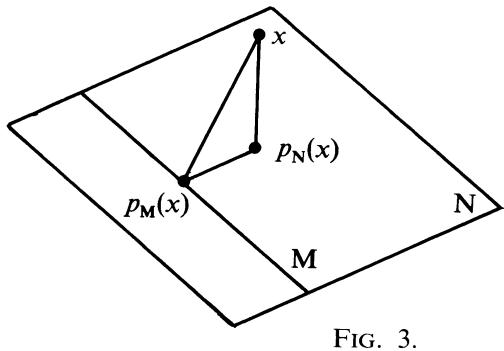
\includegraphics[keepaspectratio]{images/part002_dc4b20c6.jpg}}

\subsection{希尔伯特空间的对偶}

定理 3. --- 设 E 为希尔伯特空间。对每个 \(x \in E\) ，设 \(x^{*}\) 为 E 上的连续线性型 \(y \mapsto \langle x | y \rangle\) ；映射 \(x \mapsto x^{*}\) 是从 E 到其对偶上的一个双射的、半线性的映射（关于自同构 \(\xi \mapsto \overline{\xi}\) ），即从 E 到 \(E'\) 上，并且是从赋范空间 E 到赋范空间 \(E'\) 上的一个等距。

映射 \(x \mapsto x^*\) 由 (2)（V, p.~1）是半线性的，且由 Cauchy-Schwarz 不等式，我们有 \(\| x^* \| = \sup_{\| y \| \leqslant 1} |\langle x | y \rangle| = \| x \|\) ，故 \(x \mapsto x^*\) 是从 E 到 E' 中的一个等距，特别地是单射。为完成证明，需要证明对 E' 中所有 \(x' \neq 0\) ，存在 \(x \in E\) 使 \(x' = x^*\) 。而超平面 \(H = Ker x'\) 在 E 中是闭的；它的正交是一条直线 D。设 \(b\) 为 D 的一个非零元素；线性型 \(b^*\) 的核等于 H，因此存在标量 \(\lambda \neq 0\) 使 \(x' = \lambda . b^* = (\overline{\lambda}. b)^*\) 。证毕。

映射 \(x \mapsto x^{*}\) （从 E 到其对偶 \(E'\) 上的）称为典范映射。从 \(E'\) 到 E 上的逆映射也称为典范的，记作 \(x' \mapsto x'^{*}\) 。我们有

\[
\langle x | y \rangle = \langle y, x ^ {*} \rangle , \quad \langle x, x ^ {\prime} \rangle = \langle x ^ {\prime *} | x \rangle\tag{17}
\]

对 E 中的 \(x, y\) 与 E' 中的 \(x'\) 。还有 \((x^{*})^{*} = x\) 对 \(x \in \mathbf{E}\) 成立。

当 K 是 R 时，映射 \(x \mapsto x^{*}\) 是线性的。我们将用这个映射把 E 的内积转移到 \(E'\) 上。当 \(K = C\) 时，可以把映射 \(x \mapsto x^{*}\) 看作从向量空间 \(\overline{E}\) （E 的共轭）到 \(E'\) 上的同构（V, p.~6）。我们将用这个映射把 \(\overline{E}\) 的内积转移到 \(E'\) 上。

在所考虑的两种情形中，\(E'\) 是希尔伯特空间，且我们有公式

\[
\langle x ^ {*} | y ^ {*} \rangle = \overline {{\langle x | y \rangle}}, \quad \langle x ^ {\prime} | x ^ {\prime} \rangle = \| x ^ {\prime} \| ^ {2}
\]

对 \(x, y\) （\(\mathbf{E}\) 中的）与 \(x'\) （\(\mathbf{E}'\) 中的）。

说向量 \(x \in E\) 与向量 \(y \in E\) 正交，等价于说线性型 \(x^{*} \in E'\) 在 II, p.~41 所定义的意义下与 y 正交（这证明在两种情形下都可用«正交»一词）。若 M 是 E 的闭向量子空间，则与 M 正交的子空间 \(M^{\circ}\) （\(E'\) 中的，II, p.~44）是 E 中 M 的正交（定义于 V, p.~13）在 \(x \mapsto x^{*}\) 下的像（这证明在两种情形下都可用记号 \(M^{\circ}\)）。

推论 1. --- 为使希尔伯特空间 E 的点族 \((x_{i})_{i\in I}\) 是完全的，必要且充分的是：关系式 \(\langle x_{i}|y\rangle = 0\) （对 \(y \in E\) 且对所有指标 \(i \in I\) ）蕴含 y = 0。

事实上，这就是说 0 是 \(\mathbf{E}'\) 中与所有 \(x_{i}\) 正交的唯一的向量（II, p.~43 与 IV, p.~1）。

推论 2. --- 设 E 与 F 为两个希尔伯特空间。对 \(u \in \mathcal{L}(\mathrm{E};\mathrm{F})\) 、\(x \in \mathrm{E}\) 与 \(y \in \mathrm{F}\) ，令

\[
\Phi_ {u} (y, x) = \langle y | u (x) \rangle .\tag{18}
\]

映射 \(u \mapsto \Phi_u\) 是从 Banach 空间 \(\mathcal{L}(\mathrm{E};\mathrm{F})\) 到所有连续半双线性型 \(^1\) （\(\mathrm{F} \times \mathrm{E}\) 上的）组成的空间（赋以范数

\[
\| f\| = \sup_{\substack{x\in \mathbf{E},  y\in \mathbf{F}\\ \| x\| \leqslant 1, \| y\| \leqslant 1}}\left|f(y,x)\right|.\tag{19}
\]

显然 \(\Phi_u\) 对所有 \(u \in \mathcal{L}(\mathrm{E};\mathrm{F})\) 是半双线性的且连续的。反之，设 \(f\) 为 \(\mathrm{F} \times \mathrm{E}\) 上的连续半双线性型。对每个 \(x \in \mathrm{E}\) ，映射 \(y \mapsto \overline{f(y,x)}\) 是希尔伯特空间 \(\mathrm{F}\) 上的连续线性型。由定理 3，对每个 \(x \in \mathrm{E}\) ，存在唯一的元素 \(u(x)\) （在 \(\mathrm{F}\) 中）使 \(\overline{f(y,x)} = \langle u(x)|y\rangle\) 对所有 \(y \in \mathrm{F}\) 成立。映射 \(u: x \mapsto u(x)\) （从 \(\mathrm{E}\) 到 \(\mathrm{F}\) 中）是线性的，且我们有

\[
\begin{array}{l} \| f \| = \sup _ {\| x \| \leqslant 1} \sup _ {\| y \| \leqslant 1} | f (y, x) | = \sup _ {\| x \| \leqslant 1} \sup _ {\| y \| \leqslant 1} | \langle y | u (x) \rangle | \\ = \sup _ {\| x \| \leqslant 1} \| u (x) \|; \end{array}
\]

于是 \(u\) 属于 \(\mathcal{L}(\mathrm{E};\mathrm{F})\) ，\(f = \Phi_u\) 且 \(\| u\| = \| f\|\) 。这就证明了推论 2。

\(^{1}\) 回顾（A, IX, § 1, No.~5），F × E 上的（左）半双线性型 f 是从 F × E 到 K 中的映射，且满足 V, p.~1 的关系式 (1) 与 (2)。

从 E 到其双对偶 \(E''\) 的典范映射（IV, p.~14）把 E 映到 \(E''\) 上，换句话说（IV, p.~16），E 是自反 Banach 空间。事实上，若 E 是实（相应地，复）希尔伯特空间，则典范映射 \(\phi\) （从 \(E'\) 到 E 上的）是从赋范空间 \(E'\) 到 E（相应地，到 E 的共轭空间 \(\overline{E}\) ）上的一个同构；对 E（相应地，\(\overline{E}\) ）应用定理 3，我们看到赋范空间 \(E'\) 上的每个连续线性型都具有形式 \(x' \mapsto \langle \phi(x') | x \rangle = \langle x, x' \rangle\) ，其中 \(x \in E\) ，由此得出我们的断言。

作为推论（IV, p.~17, 命题 6）：

定理 4. --- 在希尔伯特空间 E 中，单位球是弱紧的。

命题 10. --- 若在希尔伯特空间 E 中，滤子 F 弱收敛于 \(x_{0}\) ，且又有 \(\lim_{\mathfrak{F}} \|x\| = \|x_{0}\|\) ，则 F 对 E 的初始拓扑收敛于 \(x_{0}\) 。事实上，\(\|x - x_{0}\|^{2} = \|x\|^{2} - 2R \langle x|x_{0} \rangle + \|x_{0}\|^{2}\) 。由于按假设 \(\langle x|x_{0}\rangle\) 关于 F 趋于 \(\|x_{0}\|^{2}\) ，且 \(\|x\|\) 关于 F 趋于 \(\|x_{0}\|\) ，故 \(\|x - x_{0}\|\) 关于 F 趋于 0，由此得命题。

注. --- 若 E 是 Hausdorff 准希尔伯特空间，\(\hat{E}\) 是 E 的希尔伯特空间完备化，我们知道（III, p.~16）E 的对偶 \(E'\) 可与 \(\hat{E}\) 的对偶等同；于是由定理 3（V, p.~15），E 上的每个连续线性型都可以唯一地写成 \(x \mapsto \langle a|x\rangle\) ，其中 \(a \in \hat{E}\) 。

\section{希尔伯特空间中的正交族}
